\documentclass[a4paper,12pt,twoside]{memoir}

% Castellano
\usepackage[spanish,es-tabla]{babel}
\selectlanguage{spanish}
\usepackage[utf8]{inputenc}
\usepackage[T1]{fontenc}
\usepackage{lmodern} % scalable font
\usepackage{microtype}
\usepackage{placeins}

\RequirePackage{booktabs}
\RequirePackage[table]{xcolor}
\RequirePackage{xtab}
\RequirePackage{multirow}

% Links
\PassOptionsToPackage{hyphens}{url}\usepackage[colorlinks]{hyperref}
\hypersetup{
	allcolors = {red}
}

% Ecuaciones
\usepackage{amsmath}

% Rutas de fichero / paquete
\newcommand{\ruta}[1]{{\sffamily #1}}

% Párrafos
\nonzeroparskip

% Huérfanas y viudas
\widowpenalty100000
\clubpenalty100000

% Evitar solapes en el header
\nouppercaseheads

% Imagenes
\usepackage{graphicx}
\newcommand{\imagen}[2]{
	\begin{figure}[!h]
		\centering
		\includegraphics[width=0.9\textwidth]{#1}
		\caption{#2}\label{fig:#1}
	\end{figure}
	\FloatBarrier
}

\newcommand{\imagenflotante}[2]{
	\begin{figure}%[!h]
		\centering
		\includegraphics[width=0.9\textwidth]{#1}
		\caption{#2}\label{fig:#1}
	\end{figure}
}



% El comando \figura nos permite insertar figuras comodamente, y utilizando
% siempre el mismo formato. Los parametros son:
% 1 -> Porcentaje del ancho de página que ocupará la figura (de 0 a 1)
% 2 --> Fichero de la imagen
% 3 --> Texto a pie de imagen
% 4 --> Etiqueta (label) para referencias
% 5 --> Opciones que queramos pasarle al \includegraphics
% 6 --> Opciones de posicionamiento a pasarle a \begin{figure}
\newcommand{\figuraConPosicion}[6]{%
  \setlength{\anchoFloat}{#1\textwidth}%
  \addtolength{\anchoFloat}{-4\fboxsep}%
  \setlength{\anchoFigura}{\anchoFloat}%
  \begin{figure}[#6]
    \begin{center}%
      \Ovalbox{%
        \begin{minipage}{\anchoFloat}%
          \begin{center}%
            \includegraphics[width=\anchoFigura,#5]{#2}%
            \caption{#3}%
            \label{#4}%
          \end{center}%
        \end{minipage}
      }%
    \end{center}%
  \end{figure}%
}

%
% Comando para incluir imágenes en formato apaisado (sin marco).
\newcommand{\figuraApaisadaSinMarco}[5]{%
  \begin{figure}%
    \begin{center}%
    \includegraphics[angle=90,height=#1\textheight,#5]{#2}%
    \caption{#3}%
    \label{#4}%
    \end{center}%
  \end{figure}%
}
% Para las tablas
\newcommand{\otoprule}{\midrule [\heavyrulewidth]}
%
% Nuevo comando para tablas pequeñas (menos de una página).
\newcommand{\tablaSmall}[5]{%
 \begin{table}
  \begin{center}
   \rowcolors {2}{gray!35}{}
   \begin{tabular}{#2}
    \toprule
    #4
    \otoprule
    #5
    \bottomrule
   \end{tabular}
   \caption{#1}
   \label{tabla:#3}
  \end{center}
 \end{table}
}

%
%Para el float H de tablaSmallSinColores
\usepackage{float}

%
% Nuevo comando para tablas pequeñas (menos de una página).
\newcommand{\tablaSmallSinColores}[5]{%
 \begin{table}[H]
  \begin{center}
   \begin{tabular}{#2}
    \toprule
    #4
    \otoprule
    #5
    \bottomrule
   \end{tabular}
   \caption{#1}
   \label{tabla:#3}
  \end{center}
 \end{table}
}

\newcommand{\tablaApaisadaSmall}[5]{%
\begin{landscape}
  \begin{table}
   \begin{center}
    \rowcolors {2}{gray!35}{}
    \begin{tabular}{#2}
     \toprule
     #4
     \otoprule
     #5
     \bottomrule
    \end{tabular}
    \caption{#1}
    \label{tabla:#3}
   \end{center}
  \end{table}
\end{landscape}
}

%
% Nuevo comando para tablas grandes con cabecera y filas alternas coloreadas en gris.
\newcommand{\tabla}[6]{%
  \begin{center}
    \tablefirsthead{
      \toprule
      #5
      \otoprule
    }
    \tablehead{
      \multicolumn{#3}{l}{\small\sl continúa desde la página anterior}\\
      \toprule
      #5
      \otoprule
    }
    \tabletail{
      \hline
      \multicolumn{#3}{r}{\small\sl continúa en la página siguiente}\\
    }
    \tablelasttail{
      \hline
    }
    \bottomcaption{#1}
    \rowcolors {2}{gray!35}{}
    \begin{xtabular}{#2}
      #6
      \bottomrule
    \end{xtabular}
    \label{tabla:#4}
  \end{center}
}

%
% Nuevo comando para tablas grandes con cabecera.
\newcommand{\tablaSinColores}[6]{%
  \begin{center}
    \tablefirsthead{
      \toprule
      #5
      \otoprule
    }
    \tablehead{
      \multicolumn{#3}{l}{\small\sl continúa desde la página anterior}\\
      \toprule
      #5
      \otoprule
    }
    \tabletail{
      \hline
      \multicolumn{#3}{r}{\small\sl continúa en la página siguiente}\\
    }
    \tablelasttail{
      \hline
    }
    \bottomcaption{#1}
    \begin{xtabular}{#2}
      #6
      \bottomrule
    \end{xtabular}
    \label{tabla:#4}
  \end{center}
}

%
% Nuevo comando para tablas grandes sin cabecera.
\newcommand{\tablaSinCabecera}[5]{%
  \begin{center}
    \tablefirsthead{
      \toprule
    }
    \tablehead{
      \multicolumn{#3}{l}{\small\sl continúa desde la página anterior}\\
      \hline
    }
    \tabletail{
      \hline
      \multicolumn{#3}{r}{\small\sl continúa en la página siguiente}\\
    }
    \tablelasttail{
      \hline
    }
    \bottomcaption{#1}
  \begin{xtabular}{#2}
    #5
   \bottomrule
  \end{xtabular}
  \label{tabla:#4}
  \end{center}
}



\definecolor{cgoLight}{HTML}{EEEEEE}
\definecolor{cgoExtralight}{HTML}{FFFFFF}

%
% Nuevo comando para tablas grandes sin cabecera.
\newcommand{\tablaSinCabeceraConBandas}[5]{%
  \begin{center}
    \tablefirsthead{
      \toprule
    }
    \tablehead{
      \multicolumn{#3}{l}{\small\sl continúa desde la página anterior}\\
      \hline
    }
    \tabletail{
      \hline
      \multicolumn{#3}{r}{\small\sl continúa en la página siguiente}\\
    }
    \tablelasttail{
      \hline
    }
    \bottomcaption{#1}
    \rowcolors[]{1}{cgoExtralight}{cgoLight}

  \begin{xtabular}{#2}
    #5
   \bottomrule
  \end{xtabular}
  \label{tabla:#4}
  \end{center}
}




\graphicspath{ {./img/} }

% Capítulos
\chapterstyle{bianchi}
\newcommand{\capitulo}[2]{
	\setcounter{chapter}{#1}
	\setcounter{section}{0}
	\setcounter{figure}{0}
	\setcounter{table}{0}
	\chapter*{#2}
	\addcontentsline{toc}{chapter}{#2}
	\markboth{#2}{#2}
}

% Apéndices
\renewcommand{\appendixname}{Apéndice}
\renewcommand*\cftappendixname{\appendixname}

\newcommand{\apendice}[1]{
	%\renewcommand{\thechapter}{A}
	\chapter{#1}
}

\renewcommand*\cftappendixname{\appendixname\ }

% Formato de portada
\makeatletter
\usepackage{xcolor}
\newcommand{\tutor}[1]{\def\@tutor{#1}}
\newcommand{\course}[1]{\def\@course{#1}}
\definecolor{cpardoBox}{HTML}{E6E6FF}
\def\maketitle{
  \null
  \thispagestyle{empty}
  % Cabecera ----------------
\noindent
\includegraphics[width=\textwidth]{cabecera}\vspace{1cm}%
  \vfill
  % Título proyecto y escudo informática ----------------
  \colorbox{cpardoBox}{%
    \begin{minipage}{.8\textwidth}
      \vspace{.5cm}\Large
      \begin{center}
      \textbf{TFG del Grado en Ingeniería Informática}\vspace{.6cm}\\
      \textbf{\LARGE\@title{}}
      \end{center}
      \vspace{.2cm}
    \end{minipage}

  }%
  \hfill\begin{minipage}{.20\textwidth}
    
\includegraphics[width=\textwidth]{escudoInfor}
  \end{minipage}
  \vfill
  % Datos de alumno, curso y tutores ------------------
  \begin{center}%
  {%
    \noindent\LARGE
    Presentado por \@author{}\\ 
    en Universidad de Burgos --- \@date{}\\
    Tutor: \@tutor{}\\
  }%
  \end{center}%
  \null
  \cleardoublepage
  }
\makeatother


% Datos de portada
\title{título del TFG \\Documentación Técnica}
\author{nombre alumno}
\tutor{nombre tutor}
\date{\today}

\begin{document}

\maketitle



\cleardoublepage



%%%%%%%%%%%%%%%%%%%%%%%%%%%%%%%%%%%%%%%%%%%%%%%%%%%%%%%%%%%%%%%%%%%%%%%%%%%%%%%%%%%%%%%%



\frontmatter


\clearpage

% Indices
\tableofcontents

\clearpage

\listoffigures

\clearpage

\listoftables

\clearpage

\mainmatter

\appendix

\apendice{Plan de Proyecto Software}

\section{Introducción}
En este apéndice trata el estudio de la viabilidad del proyecto y la realización de la planificación
del mismo.
\section{Planificación temporal}

\section{Estudio de viabilidad}

\subsection{Viabilidad económica}

\subsection{Viabilidad legal}



\apendice{Especificación de Requisitos}

\section{Introducción}
En esta sección se plantearán los requisitos funcionales de esta aplicación y se establecerán los casos de uso. El objetivo de este apartado es dejar una clara guía, que los desarrolladores podrán seguir para hacer un desarrollo eficiente y situado en un marco de trabajo correctamente delimitado. El diseño y planteamiento de requisitos funcionales y casos de uso son tareas cotidianas y relevantes en el desarrollo de software ya que ofrecen una guía clara de cuales son las características y funcionalidades del software que se quiere desarrollar.

\section{Objetivos generales}
Para plantear un catalogo de requisitos que ayude al diseño de casos de uso es necesario conocer los objetivos de la aplicación. Por ende, se explican en este apartado los objetivos que tiene la aplicación y las necesidades que cubre,

En primer lugar, se quiere hacer el mantenimiento de la aplicación. eLerningQA, es una aplicación que ya tiene versiones funcionales \cite{tfg-robertoArasti}, sin embargo, con las nuevas versiones de Moodle hay funcionalidades de está aplicación que fallan con las versiones de Moodle 4 y superiores. Por ende, el primer objetivo es arreglar este error, de forma que todas las funcionalidades existentes sean compatibles con las versiones de Moolde mencionadas. 

En este mantenimiento se quiere que las siguientes funcionalidades sigan siendo funcionales y compatibles con las nuevas versiones de Moodle:

\begin{itemize}
    \item \textbf{Inicio de sesión con fichero de configuración:} Se requiere poder iniciar sesión a la aplicación con una cuenta de usuario del sitio Moodle que se especifica en uno de los campos del formulario para iniciar sesión. Además, se podrá escoger entre 3 ficheros de configuración que tendrán datos para el calculo de reglas de los reportes.
    \item \textbf{Visualización de lista de cursos:} Se requiere que una vez iniciada la sesión en la aplicación se pueda visualizar una lista con los cursos a los que tiene acceso el usuario, además, el usuario debe tener permisos relativos a los de profesor o superiores. Por otro lado, el usuario,tendrá  visibles varios botones: desconexión, manual de usuario,  acerca de y contacto.
    \item \textbf{Visualización de reporte de un curso:} Cuando el usuario elige un curso de la lista, se le redirige a la página en la que visualiza el reporte del curso en cuestión. En esta pagina se le muestra un marco con todas las reglas disponibles, así como, la puntuación obtenida por cada regla ,el porcentaje obtenido en cada fase y el porcentaje total. También, se le muestra las sugerencias para mejorar la puntuación de cada regla que haya dado un resultado negativo. Estas sugerencias se pueden ver en la totalidad del curso, por cada fase o por cada regla, pulsando en la puntuación total del curso, en la puntuación de cada fase o en cada curso respectivamente. Además se le muestran varios botones: redirección al curso en la página del sitio de Moodle, redirección a la página de evolución del rendimiento y opciones de manual de usuario, acerca de, y contacto.
    \item \textbf{Visualización de la evolución de rendimiento:} En está pagina se muestra un marco con los porcentajes contextualizados en las perspectivas y los roles. Además se muestra un gráfico, con la evolución de calidad en ese curso a lo largo del tiempo. En esta página se muestran los mismo botones que en el reporte del curso.
    \item \textbf{Manual de usuario:} Se requiere poder acceder al manual de usuario, tanto si se ha iniciado la sesión como si no. En este manual se podrán ver las funcionalidades disponibles y una explicación de los contenidos.
    \item \textbf{Contacto:} Al pulsar el botón de contacto, se puede enviar un correo a la dirección de correo especificada para el contacto.
    \item \textbf{Acerca de:} Al pulsar el botón de acerca de, se podrá ver información de los autores y la licencia de la aplicación.
\end{itemize}

En segundo lugar, se quieren aumentar nuevas reglas para los reportes de los cursos. Estás reglas deben  ser relativas al diseño y realización de cuestionarios. Las reglas se basarán en estadísticas que ofrece Moodle para el estudio de calidad de cuestionarios. Cada regla implementada debe estar en la fase que le corresponde en el reporte. Además se mostrará sugerencias por cada regla con resultado negativo. Si la regla se basa en un índice que se calcula sobre cada pregunta, se mostrará una sugerencia desplegable en la que se mostrará cada índice de cada pregunta con mal índice. Si el índice sobre el que se plantea la regla se calcula para el conjunto del cuestionario, se mostrará una sugerencia simple. Las sugerencias deben tener un enlace al cuestionario en cuestión. También, se quiere añadir reglas sobre el diseño del curso. Todas estas nuevas reglas, tienen valores para su calculo en el fichero de configuración

Por otro lado, se quiere añadir una opción de exportación de reportes en Excel. Para esto se requiere tener un botón en la página de visualización del informe de un curso. Al pulsar dicho botón se descarga el fichero Excel automáticamente. En este fichero Excel se puede ver la lista con todas las reglas del reporte y los resultados de las reglas, de cada fase y la puntuación total.

\section{Catálogo de requisitos}
En este apartado se plantea el catalogo de requisitos que se pueden identificar en el apartado anterior. Con este catálogo de requisitos se podrán plantear los casos de uso. Podemos diferencia entre requisitos funcionales y no funcionales.

\subsection{Requisitos funcionales}
\begin{itemize}
    \item \textbf{RF1:} Sesión del usuario
        \begin{itemize}
            \item \textbf{RF1.1:} Incio de sesión con cuenta de usuario de Moodle
            \item \textbf{RF1.2:} Desconexión de la aplicación.
        \end{itemize}
    \item \textbf{RF2:} Lista de cursos disponibles
    \item \textbf{RF3:} Reporte de curso
        \begin{itemize}
            \item \textbf{RF3.1:} Marco con puntuaciones de las reglas definidas
            \item \textbf{RF3.2:} Marco de sugerencias para reglas fallidas
                \begin{itemize}
                    \item \textbf{RF3.2.1:} Puntuación general
                    \item \textbf{RF3.2.2:} Diseño
                    \begin{itemize}
                        \item \textbf{RF3.2.2.1:} Las opciones de progreso del estudiante están activadas
                        \item \textbf{RF3.2.2.2:} El curso tiene grupos
                        \item \textbf{RF3.2.2.3:} El curso tiene actividades grupales
                        \item \textbf{RF3.2.2.4:} Los estudiantes pueden ver las condiciones necesarias para completar una actividad
                        \item \textbf{RF3.2.2.5:} Todas las actividades tienen la misma nota máxima en el calificador
                        \item \textbf{RF3.2.2.6:} El curso tiene fechas y descripción definidas
                        \item \textbf{RF3.2.2.7:} Las preguntas de los cuestionarios tienen una calificación aleatoria adecuada
                    \end{itemize}
                    \item \textbf{RF3.2.3:} Implementación
                        \begin{itemize}
                            \item \textbf{RF3.2.3.1:} Los recursos están actualizados
                            \item \textbf{RF3.2.3.2:} Fechas de apertura y cierre de tareas son correctas
                            \item \textbf{RF3.2.3.3:} Se detallan los criterios de evaluación (rúbricas, ejemplos)
                            \item \textbf{RF3.2.3.4:} El calificador no tiene demasiado anidamiento
                            \item \textbf{RF3.2.3.5:} Todos los alumnos están en algún grupo
                        \end{itemize}
                    \item \textbf{RF3.2.4:} Realización
                        \begin{itemize}
                            \item \textbf{RF3.2.4.1:} El profesor responde en los foros dentro del límite de 48 horas lectivas desde que se plantea la duda
                            \item \textbf{RF3.2.4.2:} Se ofrece retroalimentación de las tareas
                            \item \textbf{RF3.2.4.3:} Las tareas están calificadas
                            \item \textbf{RF3.2.4.4:} El calificador muestra cómo ponderan las diferentes tareas
                            \item \textbf{RF3.2.4.5:} Los índices de facilidad de las preguntas son adecuados
                            \item \textbf{RF3.2.4.6:} Los cuestionarios tienen una participación adecuada
                            \item \textbf{RF3.2.4.7:} Las preguntas de los cuestionarios tienen un índice de discriminación adecuado
                            \item \textbf{RF3.2.4.8:} Los cuestionarios tienen un coeficiente de consistencia interna adecuado
                        \end{itemize}
                    \item \textbf{RF3.2.5:} Evaluación
                        \begin{itemize}
                            \item \textbf{RF3.2.5.1:} La mayoría de alumnos responde a los feedbacks
                            \item \textbf{RF3.2.5.2:} Se utilizan encuestas de opinión
                        \end{itemize}
                \end{itemize}
            \item \textbf{RF3.3:} Exportación a fichero Excel del reporte
            \item \textbf{RF3.4:} Redirección a página del sitio de Moodle
        \end{itemize}
    \item \textbf{RF5:} Evolución del rendimiento
        \begin{itemize}
            \item \textbf{RF5.1:} Marco con porcentajes obtenidos del cálculo entre roles y perspectivas
            \item \textbf{RF5.2:} Gráfica de evolución temporal de la calidad del curso
        \end{itemize}
    \item \textbf{RF6:} Manual de usuario
    \item \textbf{RF7:} Acerca de
    \item \textbf{RF8:} Contacto
\end{itemize}

\subsection{Requisitos no funcionales}

\begin{itemize}
    \item \textbf{RNF1 - Seguridad:} Se requiere que la aplicación haga un trato seguro a los datos introducidos por los usuarios, así como, utilizar librerías seguras y herramientas para garantizar la seguridad en la aplicación. 
    \item \textbf{RNF2 - Mantenibilidad:}  La aplicación debe ser fácilmente mantenible, utilizando herramientas y marcos de trabajo claros y con amplia documentación.
    \item \textbf{RNF3 - Disponibilidad:} La aplicación debe ser disponible y debe ofrecer su funcionalidad con normalidad siempre.
    \item \textbf{RNF4 - Compatibilidad:} La aplicación debe ser compatible con todas las versiones de Moodle, así como con la mayoría de exploradores. 
    \item \textbf{RNF5 - Escalabilidad:}  La aplicación debe ser fácilmente escalable para albergar más reglas, persistencia de datos, y un número indeterminado de usuarios.
\end{itemize}

\section{Especificación de requisitos}

% Caso de Uso 1 -> Consultar Experimentos.
\begin{table}[H]
	\centering
	\begin{tabularx}{\linewidth}{ p{0.21\columnwidth} p{0.71\columnwidth}}
		\toprule
		\textbf{CU-1}    & \textbf{Sesión del usuario}\\
		\toprule
		\textbf{Versión}              & 1.0    \\
		\textbf{Autor}                & Bilal Azar El Mourabit \\
		\textbf{Requisitos asociados} & RF1 \\
		\textbf{Descripción}          & Inicio de sesión para acceso a la aplicación y desconexión de la apliación \\
    		\textbf{Precondición}         & Disponer de una cuenta de alguna página de Moodle \\
		\textbf{Acciones}             & Entrar al sitio web\\
		\textbf{Postcondición}        & N/A \\
		\textbf{Excepciones}          & \begin{itemize}
		    \item Cuenta no válida.
            \item Sitio Moodle no existente
            \item Sesión no iniciada
		\end{itemize}\\
		\textbf{Importancia}          & Alta \\
		\bottomrule
	\end{tabularx}
	\caption{CU-1 Sesión de usuario.}
\end{table}

\begin{table}[H]
	\centering
	\begin{tabularx}{\linewidth}{ p{0.21\columnwidth} p{0.71\columnwidth} }
		\toprule
		\textbf{CU-2}    & \textbf{Incio de sesión}\\
		\toprule
		\textbf{Versión}              & 1.5    \\
		\textbf{Autor}                & Bilal Azar El Mourabit \\
		\textbf{Requisitos asociados} & RF1, RF1.1 \\
		\textbf{Descripción}          & Inicio de sesión para acceso a la aplicación \\
    		\textbf{Precondición}         & Disponer de una cuenta de alguna página de Moodle  \\
		\textbf{Acciones}             & Entrar al sitio web
		\begin{enumerate}
			\def\labelenumi{\arabic{enumi}.}
			\tightlist
			\item Rellenar los campos de usuario, contraseña, sitio de Moodle y elegir archivo de configuración
			\item Pulsar el botón de inicio de sesión
		\end{enumerate}\\
		\textbf{Postcondición}        & N/A  \\
		\textbf{Excepciones}          & \begin{itemize}
		    \item Cuenta no válida.
            \item Sitio Moodle no existente
		\end{itemize} \\
		\textbf{Importancia}          & Alta \\
		\bottomrule
	\end{tabularx}
	\caption{CU-2 Inicio de sesión.}
\end{table}

\begin{table}[H]
	\centering
	\begin{tabularx}{\linewidth}{ p{0.21\columnwidth} p{0.71\columnwidth} }
		\toprule
		\textbf{CU-3}    & \textbf{Desconexión}\\
		\toprule
		\textbf{Versión}              & 1.0    \\
		\textbf{Autor}                & Bilal Azar El Mourabit \\
		\textbf{Requisitos asociados} & RF1, RF1.2 \\
		\textbf{Descripción}          & Desconexión de la aplicación \\
    		\textbf{Precondición}         & Tener una sesión iniciada en la aplicación  \\
		\textbf{Acciones}             & 
		\begin{enumerate}
			\def\labelenumi{\arabic{enumi}.}
			\tightlist
			\item Pulsar el botón de desconexión
		\end{enumerate}\\
		\textbf{Postcondición}        & N/A \\
		\textbf{Excepciones}          & \begin{itemize}
		    \item Sesión no iniciada.
		\end{itemize} \\
		\textbf{Importancia}          & Media \\
		\bottomrule
	\end{tabularx}
	\caption{CU-3 Desconexión.}
\end{table}

\begin{table}[H]
	\centering
	\begin{tabularx}{\linewidth}{ p{0.21\columnwidth} p{0.71\columnwidth} }
		\toprule
		\textbf{CU-4}    & \textbf{Lista de cursos disponibles}\\
		\toprule
		\textbf{Versión}              & 1.0    \\
		\textbf{Autor}                & Bilal Azar El Mourabit \\
		\textbf{Requisitos asociados} & RF2 \\
		\textbf{Descripción}          & Visualización de listado de cursos disponibles \\
    		\textbf{Precondición}         & Tener una sesión iniciada en la aplicación  \\
		\textbf{Acciones}             & 
		\begin{enumerate}
			\def\labelenumi{\arabic{enumi}.}
			\tightlist
			\item Iniciar sesión
		\end{enumerate}\\
		\textbf{Postcondición}        & N/A \\
		\textbf{Excepciones}          & \begin{itemize}
		    \item Sesión no iniciada.
		\end{itemize} \\
		\textbf{Importancia}          & Media \\
		\bottomrule
	\end{tabularx}
	\caption{CU-4 Lista de cursos.}
\end{table}

\begin{table}[H]
	\centering
	\begin{tabularx}{\linewidth}{ p{0.21\columnwidth} p{0.71\columnwidth} }
		\toprule
		\textbf{CU-5}    & \textbf{Reporte de curso}\\
		\toprule
		\textbf{Versión}              & 2.0    \\
		\textbf{Autor}                & Bilal Azar El Mourabit \\
		\textbf{Requisitos asociados} & RF3 \\
		\textbf{Descripción}          & Informe de calidad completo de un curso \\
    		\textbf{Precondición}         & Tener una sesión iniciada en la aplicación  \\
		\textbf{Acciones}             & 
		\begin{enumerate}
			\def\labelenumi{\arabic{enumi}.}
			\tightlist
			\item Pulsar el enlace correspondiente al curso en la lista de cursos.
		\end{enumerate}\\
		\textbf{Postcondición}        & N/A \\
		\textbf{Excepciones}          & \begin{itemize}
		    \item Sesión no iniciada.
		\end{itemize} \\
		\textbf{Importancia}          & Alta \\
		\bottomrule
	\end{tabularx}
	\caption{CU-5 Reporte de curso}
\end{table}

\begin{table}[H]
	\centering
	\begin{tabularx}{\linewidth}{ p{0.21\columnwidth} p{0.71\columnwidth} }
		\toprule
		\textbf{CU-6}    & \textbf{Marco con puntuaciones de las reglas definidas}\\
		\toprule
		\textbf{Versión}              & 2.0   \\
		\textbf{Autor}                & Bilal Azar El Mourabit \\
		\textbf{Requisitos asociados} & RF3, RF3.1 \\
		\textbf{Descripción}          & Marco con las puntuaciones de las reglas definidas \\
    		\textbf{Precondición}         & Tener una sesión iniciada en la aplicación y acceder desde la lista de cursos  \\
		\textbf{Acciones}             & 
		\begin{enumerate}
			\def\labelenumi{\arabic{enumi}.}
			\tightlist
			\item Pulsar el enlace correspondiente al curso en la lista de cursos.
		\end{enumerate}\\
		\textbf{Postcondición}        & N/A \\
		\textbf{Excepciones}          & \begin{itemize}
		    \item Error generando el informes.
		\end{itemize} \\
		\textbf{Importancia}          & Alta \\
		\bottomrule
	\end{tabularx}
	\caption{CU-6 Marco con puntuaciones de las reglas definidas}
\end{table}

\begin{table}[H]
	\centering
	\begin{tabularx}{\linewidth}{ p{0.21\columnwidth} p{0.71\columnwidth} }
		\toprule
		\textbf{CU-7}    & \textbf{Marco de sugerencias para reglas con puntuación negativa}\\
		\toprule
		\textbf{Versión}              & 2.0    \\
		\textbf{Autor}                & Bilal Azar El Mourabit \\
		\textbf{Requisitos asociados} & RF3, RF3.2 \\
		\textbf{Descripción}          & Marco con las sugerencias de aquellas reglas que han devuelto un resultado negativo \\
    		\textbf{Precondición}         & Tener una sesión iniciada en la aplicación, acceder desde la lista de cursos y que alguna regla haya dado resultado negativo \\
		\textbf{Acciones}             & 
		\begin{enumerate}
			\def\labelenumi{\arabic{enumi}.}
			\tightlist
			\item Pulsar el enlace correspondiente al curso en la lista de cursos.
            \item Pulsar en el marco de puntuaciones la fase, la regla, o la puntución general. 
		\end{enumerate}\\
		\textbf{Postcondición}        & N/A \\
		\textbf{Excepciones}          & \begin{itemize}
		    \item Error generando el informes.
		\end{itemize} \\
		\textbf{Importancia}          & Alta \\
		\bottomrule
	\end{tabularx}
	\caption{CU-7 Marco de sugerencias para reglas con puntuación negativa}
\end{table}

\begin{table}[H]
	\centering
	\begin{tabularx}{\linewidth}{ p{0.21\columnwidth} p{0.71\columnwidth} }
		\toprule
		\textbf{CU-8}    & \textbf{Reglas de diseño}\\
		\toprule
		\textbf{Versión}              & 2.0    \\
		\textbf{Autor}                & Bilal Azar El Mourabit \\
		\textbf{Requisitos asociados} & RF3, RF3.2, RF3.2.2 \\
		\textbf{Descripción}          & Porcentaje de la media de puntuaciones de reglas de Diseño\\
    		\textbf{Precondición}         & Tener una sesión iniciada en la aplicación y permisos suficientes en la página de Moodle \\
		\textbf{Acciones}             & 
		\begin{enumerate}
			\def\labelenumi{\arabic{enumi}.}
			\tightlist
			\item Pulsar el enlace correspondiente al curso en la lista de cursos. 
		\end{enumerate}\\
		\textbf{Postcondición}        & N/A \\
		\textbf{Excepciones}          & \begin{itemize}
		    \item Error generando el informe.
		\end{itemize} \\
		\textbf{Importancia}          & Alta \\
		\bottomrule
	\end{tabularx}
	\caption{CU-8 Reglas de diseño}
\end{table}

\begin{table}[H]
	\centering
	\begin{tabularx}{\linewidth}{ p{0.21\columnwidth} p{0.71\columnwidth} }
		\toprule
		\textbf{CU-9}    & \textbf{Las opciones de progreso de estudiante están activadas}\\
		\toprule
		\textbf{Versión}              & 2.0    \\
		\textbf{Autor}                & Bilal Azar El Mourabit \\
		\textbf{Requisitos asociados} & RF3, RF3.2, RF3.2.2, RF3.2.2.1 \\
		\textbf{Descripción}          & Se comprueba que las opciones para el estudiante estén activadas\\
    		\textbf{Precondición}         & Tener una sesión iniciada en la aplicación y permisos suficientes en la página de Moodle\\
		\textbf{Acciones}             & 
		\begin{enumerate}
			\def\labelenumi{\arabic{enumi}.}
			\tightlist
			\item Iniciar sesión.
            \item Pulsar el enlace del curso en la lista de cursos. 
		\end{enumerate}\\
		\textbf{Postcondición}        & N/A \\
		\textbf{Excepciones}          & \begin{itemize}
		    \item Error generando el informe.
		\end{itemize} \\
		\textbf{Importancia}          & Alta \\
		\bottomrule
	\end{tabularx}
	\caption{CU-9 Las opciones de progreso de estudiante están activadas}
\end{table}

\begin{table}[H]
	\centering
	\begin{tabularx}{\linewidth}{ p{0.21\columnwidth} p{0.71\columnwidth} }
		\toprule
		\textbf{CU-10}    & \textbf{El curso tiene grupos}\\
		\toprule
		\textbf{Versión}              & 2.0    \\
		\textbf{Autor}                & Bilal Azar El Mourabit \\
		\textbf{Requisitos asociados} & RF3, RF3.2, RF3.2.2, RF3.2.2.2 \\
		\textbf{Descripción}          & Se comprueba que el curso tenga formados grupos de estudiantes\\
    		\textbf{Precondición}         & Tener una sesión iniciada en la aplicación y permisos suficientes en la página de Moodle \\
		\textbf{Acciones}             & 
		\begin{enumerate}
			\def\labelenumi{\arabic{enumi}.}
			\tightlist
			\item Iniciar sesión.
            \item Pulsar el enlace del curso en la lista de cursos. 
		\end{enumerate}\\
		\textbf{Postcondición}        & N/A \\
		\textbf{Excepciones}          & \begin{itemize}
		    \item Error generando el informe.
		\end{itemize} \\
		\textbf{Importancia}          & Alta \\
		\bottomrule
	\end{tabularx}
	\caption{CU-10 El curso tiene grupos}
\end{table}

\begin{table}[H]
	\centering
	\begin{tabularx}{\linewidth}{ p{0.21\columnwidth} p{0.71\columnwidth} }
		\toprule
		\textbf{CU-11}    & \textbf{El curso tiene actividades grupales}\\
		\toprule
		\textbf{Versión}              & 2.0    \\
		\textbf{Autor}                & Bilal Azar El Mourabit \\
		\textbf{Requisitos asociados} & RF3, RF3.2, RF3.2.2, RF3.2.2.3 \\
		\textbf{Descripción}          & Se comprueba que el curso tenga actividades destinadas a la realización en grupo\\
    		\textbf{Precondición}         & Tener una sesión iniciada en la aplicación y permisos suficientes en la página de Moodle \\
		\textbf{Acciones}             & 
		\begin{enumerate}
			\def\labelenumi{\arabic{enumi}.}
			\tightlist
			\item Iniciar sesión.
            \item Pulsar el enlace del curso en la lista de cursos. 
		\end{enumerate}\\
		\textbf{Postcondición}        & N/A \\
		\textbf{Excepciones}          & \begin{itemize}
		    \item Error generando el informe.
		\end{itemize} \\
		\textbf{Importancia}          & Alta \\
		\bottomrule
	\end{tabularx}
	\caption{CU-11 El curso tiene actividades grupales}
\end{table}

\begin{table}[H]
	\centering
	\begin{tabularx}{\linewidth}{ p{0.21\columnwidth} p{0.71\columnwidth} }
		\toprule
		\textbf{CU-12}    & \textbf{Los estudiantes pueden ver las condiciones necesarias para completar una actividad}\\
		\toprule
		\textbf{Versión}              & 2.0   \\
		\textbf{Autor}                & Bilal Azar El Mourabit \\
		\textbf{Requisitos asociados} & RF3, RF3.2, RF3.2.2, RF3.2.2.4 \\
		\textbf{Descripción}          & Se comprueba que los estudiantes puedan ver los requisitos necesarios para completar una actividad\\
    		\textbf{Precondición}         & Tener una sesión iniciada en la aplicación y permisos suficientes en la página de Moodle \\
		\textbf{Acciones}             & 
		\begin{enumerate}
			\def\labelenumi{\arabic{enumi}.}
			\tightlist
			\item Iniciar sesión.
            \item Pulsar el enlace del curso en la lista de cursos. 
		\end{enumerate}\\
		\textbf{Postcondición}        & N/A \\
		\textbf{Excepciones}          & \begin{itemize}
		    \item Error generando el informe.
		\end{itemize} \\
		\textbf{Importancia}          & Alta \\
		\bottomrule
	\end{tabularx}
	\caption{CU-12 Los estudiantes pueden ver las condiciones necesarias para completar una actividad}
\end{table}

\begin{table}[H]
	\centering
	\begin{tabularx}{\linewidth}{ p{0.21\columnwidth} p{0.71\columnwidth} }
		\toprule
		\textbf{CU-13}    & \textbf{Todas las actividades tienen la misma nota máxima en el calificador}\\
		\toprule
		\textbf{Versión}              & 2.0    \\
		\textbf{Autor}                & Bilal Azar El Mourabit \\
		\textbf{Requisitos asociados} & RF3, RF3.2, RF3.2.2, RF3.2.2.5 \\
		\textbf{Descripción}          & Se comprueba que las actividades diseñadas tengan la misma nota máxima en el calificador\\
    		\textbf{Precondición}         & Tener una sesión iniciada en la aplicación y permisos suficientes en la página de Moodle \\
		\textbf{Acciones}             & 
		\begin{enumerate}
			\def\labelenumi{\arabic{enumi}.}
			\tightlist
			\item Iniciar sesión.
            \item Pulsar el enlace del curso en la lista de cursos. 
		\end{enumerate}\\
		\textbf{Postcondición}        & N/A \\
		\textbf{Excepciones}          & \begin{itemize}
		    \item Error generando el informe.
		\end{itemize} \\
		\textbf{Importancia}          & Alta \\
		\bottomrule
	\end{tabularx}
	\caption{CU-13 Todas las actividades tienen la misma nota
máxima en el calificador}
\end{table}

\begin{table}[H]
	\centering
	\begin{tabularx}{\linewidth}{ p{0.21\columnwidth} p{0.71\columnwidth} }
		\toprule
		\textbf{CU-14}    & \textbf{El curso tiene fechas y descripción definidas}\\
		\toprule
		\textbf{Versión}              & 1.0    \\
		\textbf{Autor}                & Bilal Azar El Mourabit \\
		\textbf{Requisitos asociados} & RF3, RF3.2, RF3.2.2, RF3.2.2.6 \\
		\textbf{Descripción}          & Se comprueba que el curso tenga fecha de inicio, de fin y descripción definidas\\
    		\textbf{Precondición}         & Tener una sesión iniciada en la aplicación y permisos suficientes en la página de Moodle \\
		\textbf{Acciones}             & 
		\begin{enumerate}
			\def\labelenumi{\arabic{enumi}.}
			\tightlist
			\item Iniciar sesión.
            \item Pulsar el enlace del curso en la lista de cursos. 
		\end{enumerate}\\
		\textbf{Postcondición}        & N/A \\
		\textbf{Excepciones}          & \begin{itemize}
		    \item Error generando el informe.
		\end{itemize} \\
		\textbf{Importancia}          & Alta \\
		\bottomrule
	\end{tabularx}
	\caption{CU-14 El curso tiene fechas y descripción definidas}
\end{table}

\begin{table}[H]
	\centering
	\begin{tabularx}{\linewidth}{ p{0.21\columnwidth} p{0.71\columnwidth} }
		\toprule
		\textbf{CU-15}    & \textbf{Las preguntas de los cuestionarios tienen una calificación aleatoria adecuada}\\
		\toprule
		\textbf{Versión}              & 1.0    \\
		\textbf{Autor}                & Bilal Azar El Mourabit \\
		\textbf{Requisitos asociados} & RF3, RF3.2, RF3.2.2, RF3.2.2.7 \\
		\textbf{Descripción}          & Se comprueba que las preguntas de los cuestionarios tengan una calificación aleatoria por debajo del valor definido en el fichero de configuración \\
    		\textbf{Precondición}         & Tener una sesión iniciada en la aplicación y permisos suficientes en la página de Moodle \\
		\textbf{Acciones}             & 
		\begin{enumerate}
			\def\labelenumi{\arabic{enumi}.}
			\tightlist
			\item Iniciar sesión.
            \item Pulsar el enlace del curso en la lista de cursos. 
		\end{enumerate}\\
		\textbf{Postcondición}        & N/A \\
		\textbf{Excepciones}          & \begin{itemize}
		    \item Error generando el informe.
		\end{itemize} \\
		\textbf{Importancia}          & Alta \\
		\bottomrule
	\end{tabularx}
	\caption{CU-15 Las preguntas de los cuestionarios tienen una calificación aleatoria adecuada}
\end{table}

\begin{table}[H]
	\centering
	\begin{tabularx}{\linewidth}{ p{0.21\columnwidth} p{0.71\columnwidth} }
		\toprule
		\textbf{CU-16}    & \textbf{Implementación}\\
		\toprule
		\textbf{Versión}              & 2.0    \\
		\textbf{Autor}                & Bilal Azar El Mourabit \\
		\textbf{Requisitos asociados} & RF3, RF3.2, RF3.2.3 \\
		\textbf{Descripción}          & Puntuación de las reglas relativas a la fase de implementación\\
    		\textbf{Precondición}         & Tener una sesión iniciada en la aplicación y permisos suficientes en la página de Moodle \\
		\textbf{Acciones}             & 
		\begin{enumerate}
			\def\labelenumi{\arabic{enumi}.}
			\tightlist
			\item Iniciar sesión.
            \item Pulsar el enlace del curso en la lista de cursos. 
		\end{enumerate}\\
		\textbf{Postcondición}        & N/A \\
		\textbf{Excepciones}          & \begin{itemize}
		    \item Error generando el informe.
		\end{itemize} \\
		\textbf{Importancia}          & Alta \\
		\bottomrule
	\end{tabularx}
	\caption{CU-16 Implementación}
\end{table}

\begin{table}[H]
	\centering
	\begin{tabularx}{\linewidth}{ p{0.21\columnwidth} p{0.71\columnwidth} }
		\toprule
		\textbf{CU-17}    & \textbf{Los recursos están actualizados}\\
		\toprule
		\textbf{Versión}              & 2.0   \\
		\textbf{Autor}                & Bilal Azar El Mourabit \\
		\textbf{Requisitos asociados} & RF3, RF3.2, RF3.2.3, RF3.2.3.1 \\
		\textbf{Descripción}          & Se comprueba que los recursos disponibles en el curso estén actualizados\\
    		\textbf{Precondición}         & Tener una sesión iniciada en la aplicación y permisos suficientes en la página de Moodle\\
		\textbf{Acciones}             & 
		\begin{enumerate}
			\def\labelenumi{\arabic{enumi}.}
			\tightlist
			\item Iniciar sesión.
            \item Pulsar el enlace del curso en la lista de cursos. 
		\end{enumerate}\\
		\textbf{Postcondición}        & N/A \\
		\textbf{Excepciones}          & \begin{itemize}
		    \item Error generando el informe.
		\end{itemize} \\
		\textbf{Importancia}          & Alta \\
		\bottomrule
	\end{tabularx}
	\caption{CU-17  Los recursos están actualizados}
\end{table}

\begin{table}[H]
	\centering
	\begin{tabularx}{\linewidth}{ p{0.21\columnwidth} p{0.71\columnwidth} }
		\toprule
		\textbf{CU-18}    & \textbf{Fechas de apertura y cierre de tareas son correcta}\\
		\toprule
		\textbf{Versión}              & 2.0    \\
		\textbf{Autor}                & Bilal Azar El Mourabit \\
		\textbf{Requisitos asociados} & RF3, RF3.2, RF3.2.3, RF3.2.3.2 \\
		\textbf{Descripción}          & Se comprueba que las fechas de apertura y cierre de los módulos estén definidos y dentro de las fechas de inicio y fin del curso\\
    		\textbf{Precondición}         & Tener una sesión iniciada en la aplicación y permisos suficientes en la página de Moodle\\
		\textbf{Acciones}             & 
		\begin{enumerate}
			\def\labelenumi{\arabic{enumi}.}
			\tightlist
			\item Iniciar sesión.
            \item Pulsar el enlace del curso en la lista de cursos. 
		\end{enumerate}\\
		\textbf{Postcondición}        & N/A \\
		\textbf{Excepciones}          & \begin{itemize}
		    \item Error generando el informe.
		\end{itemize} \\
		\textbf{Importancia}          & Alta \\
		\bottomrule
	\end{tabularx}
	\caption{CU-18 Fechas de apertura y cierre de tareas son
correcta}
\end{table}

\begin{table}[H]
	\centering
	\begin{tabularx}{\linewidth}{ p{0.21\columnwidth} p{0.71\columnwidth} }
		\toprule
		\textbf{CU-19}    & \textbf{Se detallan los criterios de evaluación (rúbricas, ejemplos)}\\
		\toprule
		\textbf{Versión}              & 2.0    \\
		\textbf{Autor}                & Bilal Azar El Mourabit \\
		\textbf{Requisitos asociados} & RF3, RF3.2, RF3.2.3, RF3.2.3.3 \\
		\textbf{Descripción}          & Se comprueba que los criterios de evaluación estén detallados\\
    		\textbf{Precondición}         & Tener una sesión iniciada en la aplicación y permisos suficientes en la página de Moodle\\
		\textbf{Acciones}             & 
		\begin{enumerate}
			\def\labelenumi{\arabic{enumi}.}
			\tightlist
			\item Iniciar sesión.
            \item Pulsar el enlace del curso en la lista de cursos. 
		\end{enumerate}\\
		\textbf{Postcondición}        & N/A \\
		\textbf{Excepciones}          & \begin{itemize}
		    \item Error generando el informe.
		\end{itemize} \\
		\textbf{Importancia}          & Alta \\
		\bottomrule
	\end{tabularx}
	\caption{CU-19 Se detallan los criterios de evaluación (rúbricas, ejemplos)}
\end{table}

\begin{table}[H]
	\centering
	\begin{tabularx}{\linewidth}{ p{0.21\columnwidth} p{0.71\columnwidth} }
		\toprule
		\textbf{CU-20}    & \textbf{El calificador no tiene demasiado anidamiento}\\
		\toprule
		\textbf{Versión}              & 2.0    \\
		\textbf{Autor}                & Bilal Azar El Mourabit \\
		\textbf{Requisitos asociados} & RF3, RF3.2, RF3.2.3, RF3.2.3.4 \\
		\textbf{Descripción}          & Se comprueba que el calificador del curso no tenga demsaiado anidamiento\\
    		\textbf{Precondición}         & Tener una sesión iniciada en la aplicación y permisos suficientes en la página de Moodle\\
		\textbf{Acciones}             & 
		\begin{enumerate}
			\def\labelenumi{\arabic{enumi}.}
			\tightlist
			\item Iniciar sesión.
            \item Pulsar el enlace del curso en la lista de cursos. 
		\end{enumerate}\\
		\textbf{Postcondición}        & N/A \\
		\textbf{Excepciones}          & \begin{itemize}
		    \item Error generando el informe.
		\end{itemize} \\
		\textbf{Importancia}          & Alta \\
		\bottomrule
	\end{tabularx}
	\caption{CU-20 El calificador no tiene demasiado anidamiento}
\end{table}

\begin{table}[H]
	\centering
	\begin{tabularx}{\linewidth}{ p{0.21\columnwidth} p{0.71\columnwidth} }
		\toprule
		\textbf{CU-21}    & \textbf{Todos los alumnos están en algún grupo}\\
		\toprule
		\textbf{Versión}              & 2.0    \\
		\textbf{Autor}                & Bilal Azar El Mourabit \\
		\textbf{Requisitos asociados} & RF3, RF3.2, RF3.2.3, RF3.2.3.5 \\
		\textbf{Descripción}          & Se comprueba que los alumnos matriculados estén en algún grupo\\
    		\textbf{Precondición}         & Tener una sesión iniciada en la aplicación y permisos suficientes en la página de Moodle\\
		\textbf{Acciones}             & 
		\begin{enumerate}
			\def\labelenumi{\arabic{enumi}.}
			\tightlist
			\item Iniciar sesión.
            \item Pulsar el enlace del curso en la lista de cursos. 
		\end{enumerate}\\
		\textbf{Postcondición}        & N/A \\
		\textbf{Excepciones}          & \begin{itemize}
		    \item Error generando el informe.
		\end{itemize} \\
		\textbf{Importancia}          & Alta \\
		\bottomrule
	\end{tabularx}
	\caption{CU-21 Todos los alumnos están en algún grupo}
\end{table}

\begin{table}[H]
	\centering
	\begin{tabularx}{\linewidth}{ p{0.21\columnwidth} p{0.71\columnwidth} }
		\toprule
		\textbf{CU-21}    & \textbf{Todos los alumnos están en algún grupo}\\
		\toprule
		\textbf{Versión}              & 2.0    \\
		\textbf{Autor}                & Bilal Azar El Mourabit \\
		\textbf{Requisitos asociados} & RF3, RF3.2, RF3.2.3, RF3.2.3.5 \\
		\textbf{Descripción}          & Se comprueba que los alumnos matriculados estén en algún grupo\\
    		\textbf{Precondición}         & Tener una sesión iniciada en la aplicación y permisos suficientes en la página de Moodle\\
		\textbf{Acciones}             & 
		\begin{enumerate}
			\def\labelenumi{\arabic{enumi}.}
			\tightlist
			\item Iniciar sesión.
            \item Pulsar el enlace del curso en la lista de cursos. 
		\end{enumerate}\\
		\textbf{Postcondición}        & N/A \\
		\textbf{Excepciones}          & \begin{itemize}
		    \item Error generando el informe.
		\end{itemize} \\
		\textbf{Importancia}          & Alta \\
		\bottomrule
	\end{tabularx}
	\caption{CU-21 Todos los alumnos están en algún grupo}
\end{table}

\begin{table}[H]
	\centering
	\begin{tabularx}{\linewidth}{ p{0.21\columnwidth} p{0.71\columnwidth} }
		\toprule
		\textbf{CU-22}    & \textbf{Realización}\\
		\toprule
		\textbf{Versión}              & 2.0    \\
		\textbf{Autor}                & Bilal Azar El Mourabit \\
		\textbf{Requisitos asociados} & RF3, RF3.2, RF3.2.4 \\
		\textbf{Descripción}          & Puntuación de las reglas relativas a la fase de implementación\\
    		\textbf{Precondición}         & Tener una sesión iniciada en la aplicación y permisos suficientes en la página de Moodle\\
		\textbf{Acciones}             & 
		\begin{enumerate}
			\def\labelenumi{\arabic{enumi}.}
			\tightlist
			\item Iniciar sesión.
            \item Pulsar el enlace del curso en la lista de cursos. 
		\end{enumerate}\\
		\textbf{Postcondición}        & N/A \\
		\textbf{Excepciones}          & \begin{itemize}
		    \item Error generando el informe.
		\end{itemize} \\
		\textbf{Importancia}          & Alta \\
		\bottomrule
	\end{tabularx}
	\caption{CU-22 Realización}
\end{table}

\begin{table}[H]
	\centering
	\begin{tabularx}{\linewidth}{ p{0.21\columnwidth} p{0.71\columnwidth} }
		\toprule
		\textbf{CU-23}    & \textbf{El profesor responde en los foros dentro del límite de 48 horas lectivas desde que se plantea la duda}\\
		\toprule
		\textbf{Versión}              & 2.0    \\
		\textbf{Autor}                & Bilal Azar El Mourabit \\
		\textbf{Requisitos asociados} & RF3, RF3.2, RF3.2.4, RF3.2.4.1 \\
		\textbf{Descripción}          & Se comprueba que las dudas planteadas por el profesor sean respondidas en 48 horas por el profesor\\
    		\textbf{Precondición}         & Tener una sesión iniciada en la aplicación y permisos suficientes en la página de Moodle\\
		\textbf{Acciones}             & 
		\begin{enumerate}
			\def\labelenumi{\arabic{enumi}.}
			\tightlist
			\item Iniciar sesión.
            \item Pulsar el enlace del curso en la lista de cursos. 
		\end{enumerate}\\
		\textbf{Postcondición}        & N/A \\
		\textbf{Excepciones}          & \begin{itemize}
		    \item Error generando el informe.
		\end{itemize} \\
		\textbf{Importancia}          & Alta \\
		\bottomrule
	\end{tabularx}
	\caption{CU-23 El profesor responde en los foros dentro del
límite de 48 horas lectivas desde que se plantea la duda}
\end{table}

\begin{table}[H]
	\centering
	\begin{tabularx}{\linewidth}{ p{0.21\columnwidth} p{0.71\columnwidth} }
		\toprule
		\textbf{CU-24}    & \textbf{Se ofrece retroalimentación de las tarea}\\
		\toprule
		\textbf{Versión}              & 2.0   \\
		\textbf{Autor}                & Bilal Azar El Mourabit \\
		\textbf{Requisitos asociados} & RF3, RF3.2, RF3.2.4, RF3.2.4.2 \\
		\textbf{Descripción}          & Se comprueba que las tareas tengan reatroalimentación por parte de los profesores\\
    		\textbf{Precondición}         & Tener una sesión iniciada en la aplicación y permisos suficientes en la página de Moodle\\
		\textbf{Acciones}             & 
		\begin{enumerate}
			\def\labelenumi{\arabic{enumi}.}
			\tightlist
			\item Iniciar sesión.
            \item Pulsar el enlace del curso en la lista de cursos. 
		\end{enumerate}\\
		\textbf{Postcondición}        & N/A \\
		\textbf{Excepciones}          & \begin{itemize}
		    \item Error generando el informe.
		\end{itemize} \\
		\textbf{Importancia}          & Alta \\
		\bottomrule
	\end{tabularx}
	\caption{CU-24 Se ofrece retroalimentación de las tarea}
\end{table}

\begin{table}[H]
	\centering
	\begin{tabularx}{\linewidth}{ p{0.21\columnwidth} p{0.71\columnwidth} }
		\toprule
		\textbf{CU-25}    & \textbf{Las tareas están calificadas}\\
		\toprule
		\textbf{Versión}              & 2.0    \\
		\textbf{Autor}                & Bilal Azar El Mourabit \\
		\textbf{Requisitos asociados} & RF3, RF3.2, RF3.2.4, RF3.2.4.3 \\
		\textbf{Descripción}          & Se comprueba que las tareas finalizadas estén calificadas\\
    		\textbf{Precondición}         & Tener una sesión iniciada en la aplicación y permisos suficientes en la página de Moodle\\
		\textbf{Acciones}             & 
		\begin{enumerate}
			\def\labelenumi{\arabic{enumi}.}
			\tightlist
			\item Iniciar sesión.
            \item Pulsar el enlace del curso en la lista de cursos. 
		\end{enumerate}\\
		\textbf{Postcondición}        & N/A \\
		\textbf{Excepciones}          & \begin{itemize}
		    \item Error generando el informe.
		\end{itemize} \\
		\textbf{Importancia}          & Alta \\
		\bottomrule
	\end{tabularx}
	\caption{CU-25 Se ofrece retroalimentación de las tarea}
\end{table}

\begin{table}[H]
	\centering
	\begin{tabularx}{\linewidth}{ p{0.21\columnwidth} p{0.71\columnwidth} }
		\toprule
		\textbf{CU-26}    & \textbf{El calificador muestra cómo ponderan las diferentes tareas}\\
		\toprule
		\textbf{Versión}              & 2.0    \\
		\textbf{Autor}                & Bilal Azar El Mourabit \\
		\textbf{Requisitos asociados} & RF3, RF3.2, RF3.2.4, RF3.2.4.4 \\
		\textbf{Descripción}          & Se comprueba que en el calificador se muestren las ponderaciones de todas las actividades\\
    		\textbf{Precondición}         & Tener una sesión iniciada en la aplicación y permisos suficientes en la página de Moodle\\
		\textbf{Acciones}             & 
		\begin{enumerate}
			\def\labelenumi{\arabic{enumi}.}
			\tightlist
			\item Iniciar sesión.
            \item Pulsar el enlace del curso en la lista de cursos. 
		\end{enumerate}\\
		\textbf{Postcondición}        & N/A \\
		\textbf{Excepciones}          & \begin{itemize}
		    \item Error generando el informe.
		\end{itemize} \\
		\textbf{Importancia}          & Alta \\
		\bottomrule
	\end{tabularx}
	\caption{CU-26 El calificador muestra cómo ponderan las diferentes tareas}
\end{table}

\begin{table}[H]
	\centering
	\begin{tabularx}{\linewidth}{ p{0.21\columnwidth} p{0.71\columnwidth} }
		\toprule
		\textbf{CU-27}    & \textbf{Los índices de facilidad de las preguntas son adecuados}\\
		\toprule
		\textbf{Versión}              & 1.0    \\
		\textbf{Autor}                & Bilal Azar El Mourabit \\
		\textbf{Requisitos asociados} & RF3, RF3.2, RF3.2.4, RF3.2.4.5 \\
		\textbf{Descripción}          & Se comprueba que las preguntas de los cuestionarios tengan un índice de facilidad comprendido en un intervalo definido en el fichero de configuración\\
    		\textbf{Precondición}         & Tener una sesión iniciada en la aplicación y permisos suficientes en la página de Moodle\\
		\textbf{Acciones}             & 
		\begin{enumerate}
			\def\labelenumi{\arabic{enumi}.}
			\tightlist
			\item Iniciar sesión.
            \item Pulsar el enlace del curso en la lista de cursos. 
		\end{enumerate}\\
		\textbf{Postcondición}        & N/A \\
		\textbf{Excepciones}          & \begin{itemize}
		    \item Error generando el informe.
		\end{itemize} \\
		\textbf{Importancia}          & Alta \\
		\bottomrule
	\end{tabularx}
	\caption{CU-27 El calificador muestra cómo ponderan las diferentes tareas}
\end{table}

\begin{table}[H]
	\centering
	\begin{tabularx}{\linewidth}{ p{0.21\columnwidth} p{0.71\columnwidth} }
		\toprule
		\textbf{CU-28}    & \textbf{Los cuestionarios tienen una participación
adecuada}\\
		\toprule
		\textbf{Versión}              & 1.0    \\
		\textbf{Autor}                & Bilal Azar El Mourabit \\
		\textbf{Requisitos asociados} & RF3, RF3.2, RF3.2.4, RF3.2.4.6 \\
		\textbf{Descripción}          & Se comprueba que los cuestionarios tengan una participación superior al valor definido en el fichero de configuración\\
    		\textbf{Precondición}         & Tener una sesión iniciada en la aplicación y permisos suficientes en la página de Moodle\\
		\textbf{Acciones}             & 
		\begin{enumerate}
			\def\labelenumi{\arabic{enumi}.}
			\tightlist
			\item Iniciar sesión.
            \item Pulsar el enlace del curso en la lista de cursos. 
		\end{enumerate}\\
		\textbf{Postcondición}        & N/A \\
		\textbf{Excepciones}          & \begin{itemize}
		    \item Error generando el informe.
		\end{itemize} \\
		\textbf{Importancia}          & Alta \\
		\bottomrule
	\end{tabularx}
	\caption{CU-28 Los cuestionarios tienen una participación
adecuada}
\end{table}

\begin{table}[H]
	\centering
	\begin{tabularx}{\linewidth}{ p{0.21\columnwidth} p{0.71\columnwidth} }
		\toprule
		\textbf{CU-29}    & \textbf{Los cuestionarios tienen una participación adecuada}\\
		\toprule
		\textbf{Versión}              & 1.0    \\
		\textbf{Autor}                & Bilal Azar El Mourabit \\
		\textbf{Requisitos asociados} & RF3, RF3.2, RF3.2.4, RF3.2.4.7 \\
		\textbf{Descripción}          & Se comprueba que las preguntas de los cuestionarios tengan un índice de discriminación superior al valor definido en el fichero de configuración\\
    		\textbf{Precondición}         & Tener una sesión iniciada en la aplicación y permisos suficientes en la página de Moodle\\
		\textbf{Acciones}             & 
		\begin{enumerate}
			\def\labelenumi{\arabic{enumi}.}
			\tightlist
			\item Iniciar sesión.
            \item Pulsar el enlace del curso en la lista de cursos. 
		\end{enumerate}\\
		\textbf{Postcondición}        & N/A \\
		\textbf{Excepciones}          & \begin{itemize}
		    \item Error generando el informe.
		\end{itemize} \\
		\textbf{Importancia}          & Alta \\
		\bottomrule
	\end{tabularx}
	\caption{CU-29 Los cuestionarios tienen una participación
adecuada}
\end{table}

\begin{table}[H]
	\centering
	\begin{tabularx}{\linewidth}{ p{0.21\columnwidth} p{0.71\columnwidth} }
		\toprule
		\textbf{CU-30}    & \textbf{Los cuestionarios tienen un coeficiente de consistencia interna adecuado}\\
		\toprule
		\textbf{Versión}              & 1.0    \\
		\textbf{Autor}                & Bilal Azar El Mourabit \\
		\textbf{Requisitos asociados} & RF3, RF3.2, RF3.2.4, RF3.2.4.8 \\
		\textbf{Descripción}          & Se comprueba que el coeficiente de consistencia interna esté por encima de un valor definido en el fichero de configuración\\
    		\textbf{Precondición}         & Tener una sesión iniciada en la aplicación y permisos suficientes en la página de Moodle\\
		\textbf{Acciones}             & 
		\begin{enumerate}
			\def\labelenumi{\arabic{enumi}.}
			\tightlist
			\item Iniciar sesión.
            \item Pulsar el enlace del curso en la lista de cursos. 
		\end{enumerate}\\
		\textbf{Postcondición}        & N/A \\
		\textbf{Excepciones}          & \begin{itemize}
		    \item Error generando el informe.
		\end{itemize} \\
		\textbf{Importancia}          & Alta \\
		\bottomrule
	\end{tabularx}
	\caption{CU-30 Los cuestionarios tienen una participación
adecuada}
\end{table}

\begin{table}[H]
	\centering
	\begin{tabularx}{\linewidth}{ p{0.21\columnwidth} p{0.71\columnwidth} }
		\toprule
		\textbf{CU-31}    & \textbf{Evaluación}\\
		\toprule
		\textbf{Versión}              & 1.0    \\
		\textbf{Autor}                & Bilal Azar El Mourabit \\
		\textbf{Requisitos asociados} & RF3, RF3.2, RF3.2.5\\
		\textbf{Descripción}          & Porcentaje de la media de las puntuaciones relativas a la fase de evaluación\\
    		\textbf{Precondición}         & Tener una sesión iniciada en la aplicación y permisos suficientes en la página de Moodle\\
		\textbf{Acciones}             & 
		\begin{enumerate}
			\def\labelenumi{\arabic{enumi}.}
			\tightlist
			\item Iniciar sesión.
            \item Pulsar el enlace del curso en la lista de cursos. 
		\end{enumerate}\\
		\textbf{Postcondición}        & N/A \\
		\textbf{Excepciones}          & \begin{itemize}
		    \item Error generando el informe.
		\end{itemize} \\
		\textbf{Importancia}          & Alta \\
		\bottomrule
	\end{tabularx}
	\caption{CU-31 Evaluación}
\end{table}

\begin{table}[H]
	\centering
	\begin{tabularx}{\linewidth}{ p{0.21\columnwidth} p{0.71\columnwidth} }
		\toprule
		\textbf{CU-32}    & \textbf{La mayoría de alumnos responde a los feedbacks}\\
		\toprule
		\textbf{Versión}              & 1.0    \\
		\textbf{Autor}                & Bilal Azar El Mourabit \\
		\textbf{Requisitos asociados} & RF3, RF3.2, RF3.2.5, RF3.2.5.1\\
		\textbf{Descripción}          & Se comprueba que la mayoría de alumnos responde a los feedbacks proporcionados\\
    		\textbf{Precondición}         & Tener una sesión iniciada en la aplicación y permisos suficientes en la página de Moodle\\
		\textbf{Acciones}             & 
		\begin{enumerate}
			\def\labelenumi{\arabic{enumi}.}
			\tightlist
			\item Iniciar sesión.
            \item Pulsar el enlace del curso en la lista de cursos. 
		\end{enumerate}\\
		\textbf{Postcondición}        & N/A \\
		\textbf{Excepciones}          & \begin{itemize}
		    \item Error generando el informe.
		\end{itemize} \\
		\textbf{Importancia}          & Alta \\
		\bottomrule
	\end{tabularx}
	\caption{CU-32 Evaluación}
\end{table}

\begin{table}[H]
	\centering
	\begin{tabularx}{\linewidth}{ p{0.21\columnwidth} p{0.71\columnwidth} }
		\toprule
		\textbf{CU-33}    & \textbf{Se utilizan encuestas de opinión}\\
		\toprule
		\textbf{Versión}              & 1.0    \\
		\textbf{Autor}                & Bilal Azar El Mourabit \\
		\textbf{Requisitos asociados} & RF3, RF3.2, RF3.2.5, RF3.2.5.2\\
		\textbf{Descripción}          & Se comprueba que en  el curso haya definidos y se utilicen encuestas de opinión\\
    		\textbf{Precondición}         & Tener una sesión iniciada en la aplicación y permisos suficientes en la página de Moodle\\
		\textbf{Acciones}             & 
		\begin{enumerate}
			\def\labelenumi{\arabic{enumi}.}
			\tightlist
			\item Iniciar sesión.
            \item Pulsar el enlace del curso en la lista de cursos. 
		\end{enumerate}\\
		\textbf{Postcondición}        & N/A \\
		\textbf{Excepciones}          & \begin{itemize}
		    \item Error generando el informe.
		\end{itemize} \\
		\textbf{Importancia}          & Alta \\
		\bottomrule
	\end{tabularx}
	\caption{CU-33 Se utilizan encuestas de opinión}
\end{table}

\begin{table}[H]
	\centering
	\begin{tabularx}{\linewidth}{ p{0.21\columnwidth} p{0.71\columnwidth} }
		\toprule
		\textbf{CU-34}    & \textbf{Exportación a fichero Excel del reporte}\\
		\toprule
		\textbf{Versión}              & 1.0    \\
		\textbf{Autor}                & Bilal Azar El Mourabit \\
		\textbf{Requisitos asociados} & RF3, RF3.3\\
		\textbf{Descripción}          & Se descraga un fichero excel con el resumen del reporte generado\\
    		\textbf{Precondición}         & Tener una sesión iniciada en la aplicación y permisos suficientes en la página de Moodle\\
		\textbf{Acciones}             & 
		\begin{enumerate}
			\def\labelenumi{\arabic{enumi}.}
			\tightlist
			\item Iniciar sesión.
            \item Pulsar el enlace del curso en la lista de cursos.
            \item Pulsar el botón de exportación de excel
		\end{enumerate}\\
		\textbf{Postcondición}        & N/A \\
		\textbf{Excepciones}          & \begin{itemize}
		    \item Error generando el informes.
		\end{itemize} \\
		\textbf{Importancia}          & Alta \\
		\bottomrule
	\end{tabularx}
	\caption{CU-34 Exportación a fichero Excel del reporte}
\end{table}

\begin{table}[H]
	\centering
	\begin{tabularx}{\linewidth}{ p{0.21\columnwidth} p{0.71\columnwidth} }
		\toprule
		\textbf{CU-35}    & \textbf{Redirección a página del sitio de Moodle}\\
		\toprule
		\textbf{Versión}              & 1.0    \\
		\textbf{Autor}                & Bilal Azar El Mourabit \\
		\textbf{Requisitos asociados} & RF3, RF3.4\\
		\textbf{Descripción}          & Se redirige a la página del curso de Moodle\\
    		\textbf{Precondición}         & Tener una sesión iniciada en la aplicación y permisos suficientes en la página de Moodle\\
		\textbf{Acciones}             & 
		\begin{enumerate}
			\def\labelenumi{\arabic{enumi}.}
			\tightlist
			\item Iniciar sesión.
            \item Pulsar el enlace del curso en la lista de cursos.
            \item Pulsar el botón con el nombre del curso
		\end{enumerate}\\
		\textbf{Postcondición}        & N/A \\
		\textbf{Excepciones}          & \begin{itemize}
		    \item Error generando el informe.
		\end{itemize} \\
		\textbf{Importancia}          & Alta \\
		\bottomrule
	\end{tabularx}
	\caption{CU-35 Redirección a página del sitio de Moodle}
\end{table}

\begin{table}[H]
	\centering
	\begin{tabularx}{\linewidth}{ p{0.21\columnwidth} p{0.71\columnwidth} }
		\toprule
		\textbf{CU-36}    & \textbf{Evolución del rendimiento}\\
		\toprule
		\textbf{Versión}              & 2.0    \\
		\textbf{Autor}                & Bilal Azar El Mourabit \\
		\textbf{Requisitos asociados} & RF5\\
		\textbf{Descripción}          & Se muestra la evolución de calidad y la puntuación de las reglas entre roles y perspectivas\\
    		\textbf{Precondición}         & Tener una sesión iniciada en la aplicación y permisos suficientes en la página de Moodle\\
		\textbf{Acciones}             & 
		\begin{enumerate}
			\def\labelenumi{\arabic{enumi}.}
			\tightlist
			\item Iniciar sesión.
            \item Pulsar el enlace del curso en la lista de cursos.
            \item Pulsar el botón de enlace de evolución rendimiento
		\end{enumerate}\\
		\textbf{Postcondición}        & N/A \\
		\textbf{Excepciones}          & \begin{itemize}
		    \item Error generando el informe.
		\end{itemize} \\
		\textbf{Importancia}          & Alta \\
		\bottomrule
	\end{tabularx}
	\caption{CU-36 Evolución del rendimiento}
\end{table}

\begin{table}[H]
	\centering
	\begin{tabularx}{\linewidth}{ p{0.21\columnwidth} p{0.71\columnwidth} }
		\toprule
		\textbf{CU-37}    & \textbf{Marco con porcentajes obtenidos del cálculo entre roles y perspectivas}\\
		\toprule
		\textbf{Versión}              & 2.0   \\
		\textbf{Autor}                & Bilal Azar El Mourabit \\
		\textbf{Requisitos asociados} & RF5, RF5.1\\
		\textbf{Descripción}          & Se muestra un marco con las puntuaciones de las reglas en las dimensiones de roles y perspectivas\\
    		\textbf{Precondición}         & Tener una sesión iniciada en la aplicación y permisos suficientes en la página de Moodle\\
		\textbf{Acciones}             & 
		\begin{enumerate}
			\def\labelenumi{\arabic{enumi}.}
			\tightlist
			\item Iniciar sesión.
            \item Pulsar el enlace del curso en la lista de cursos.
            \item Pulsar el botón de enlace de evolución rendimiento
		\end{enumerate}\\
		\textbf{Postcondición}        & N/A \\
		\textbf{Excepciones}          & \begin{itemize}
		    \item Error generando el informe.
		\end{itemize} \\
		\textbf{Importancia}          & Media \\
		\bottomrule
	\end{tabularx}
	\caption{CU-37 Evolución del rendimiento}
\end{table}

\begin{table}[H]
	\centering
	\begin{tabularx}{\linewidth}{ p{0.21\columnwidth} p{0.71\columnwidth} }
		\toprule
		\textbf{CU-38}    & \textbf{Gráfica de evolución temporal de la calidad del curso}\\
		\toprule
		\textbf{Versión}              & 1.0    \\
		\textbf{Autor}                & Bilal Azar El Mourabit \\
		\textbf{Requisitos asociados} & RF5, RF5.2\\
		\textbf{Descripción}          & Se muestra una gráfica con la evolución de calidad del curso\\
    		\textbf{Precondición}         & Tener una sesión iniciada en la aplicación y permisos suficientes en la página de Moodle\\
		\textbf{Acciones}             & 
		\begin{enumerate}
			\def\labelenumi{\arabic{enumi}.}
			\tightlist
			\item Iniciar sesión.
            \item Pulsar el enlace del curso en la lista de cursos.
            \item Pulsar el botón de enlace de evolución rendimiento
		\end{enumerate}\\
		\textbf{Postcondición}        & N/A \\
		\textbf{Excepciones}          & \begin{itemize}
		    \item Error generando el informe.
		\end{itemize} \\
		\textbf{Importancia}          & Media \\
		\bottomrule
	\end{tabularx}
	\caption{CU-38 Gráfica de evolución temporal de la calidad del curso}
\end{table}

\begin{table}[H]
	\centering
	\begin{tabularx}{\linewidth}{ p{0.21\columnwidth} p{0.71\columnwidth} }
		\toprule
		\textbf{CU-38}    & \textbf{Manual de usuario}\\
		\toprule
		\textbf{Versión}              & 2.0    \\
		\textbf{Autor}                & Bilal Azar El Mourabit \\
		\textbf{Requisitos asociados} & RF6\\
		\textbf{Descripción}          & Se muestra un manual de usuario con una descripción de todas las funcionalidades\\
    		\textbf{Precondición}         & N/A\\
		\textbf{Acciones}             & 
		\begin{enumerate}
			\def\labelenumi{\arabic{enumi}.}
			\tightlist
			\item Pulsar el botón de manual de usuario.
		\end{enumerate}\\
		\textbf{Postcondición}        & N/A \\
		\textbf{Excepciones}          & \\
		\textbf{Importancia}          & Baja \\
		\bottomrule
	\end{tabularx}
	\caption{CU-38 Gráfica de evolución temporal de la calidad del curso}
\end{table}

\begin{table}[H]
	\centering
	\begin{tabularx}{\linewidth}{ p{0.21\columnwidth} p{0.71\columnwidth} }
		\toprule
		\textbf{CU-39}    & \textbf{Acerca de}\\
		\toprule
		\textbf{Versión}              & 2.0    \\
		\textbf{Autor}                & Bilal Azar El Mourabit \\
		\textbf{Requisitos asociados} & RF7\\
		\textbf{Descripción}          & Se muestran información relativa a autores y licencias de la aplicación\\
    		\textbf{Precondición}         & N/A\\
		\textbf{Acciones}             & 
		\begin{enumerate}
			\def\labelenumi{\arabic{enumi}.}
			\tightlist
			\item Pulsar botón de acerca de.
		\end{enumerate}\\
		\textbf{Postcondición}        & N/A \\
		\textbf{Excepciones}          & \\
		\textbf{Importancia}          & Baja \\
		\bottomrule
	\end{tabularx}
	\caption{CU-39 Gráfica de evolución temporal de la calidad del curso}
\end{table}

\begin{table}[H]
	\centering
	\begin{tabularx}{\linewidth}{ p{0.21\columnwidth} p{0.71\columnwidth} }
		\toprule
		\textbf{CU-40}    & \textbf{Contacto}\\
		\toprule
		\textbf{Versión}              & 2.0    \\
		\textbf{Autor}                & Bilal Azar El Mourabit \\
		\textbf{Requisitos asociados} & RF8\\
		\textbf{Descripción}          & Se muestra un marco emergente para enviar un correo a una dirección de contacto\\
    		\textbf{Precondición}         & N/A\\
		\textbf{Acciones}             & 
		\begin{enumerate}
			\def\labelenumi{\arabic{enumi}.}
			\tightlist
			\item Pulsar botón de contacto.
		\end{enumerate}\\
		\textbf{Postcondición}        & N/A \\
		\textbf{Excepciones}          &  \\
		\textbf{Importancia}          & Baja \\
		\bottomrule
	\end{tabularx}
	\caption{CU-40 Contacto}
\end{table}
\apendice{Especificación de diseño}

\section{Introducción}
Tras haber definido los requisitos de la aplicación, es hora de definir el diseño de la aplicación. En este apartado se dará una descripción del diseño de los datos, el flujo de procedimientos y el diseño arquitectónico de la aplicación.

\section{Diseño arquitectónico}
Esta aplicación cuenta con una arquitectura Modelo-Vista-Controlador \cite{mvc}. Este es un patrón arquitectónico que divide la aplicación en tres componentes \ref{fig:mvc}:
\begin{itemize}
    \item \textbf{Modelo:} En este componente se encuentran los datos y toda la lógica relativa a su obtención.
    \item \textbf{Vista:} En la vista se encuentra la interfaz gráfica y todos aquellos componentes que interactúen directamente con el usuario.
    \item \textbf{Controlador:}Este componente es el intermediario entre el modelo y la vista, este es el que gestiona las peticiones que se reciben de la vista y decide que datos mostrar y como, es decir, es el que contiene la lógica de negocio.
\end{itemize}

\begin{figure}[H]
    \centering
    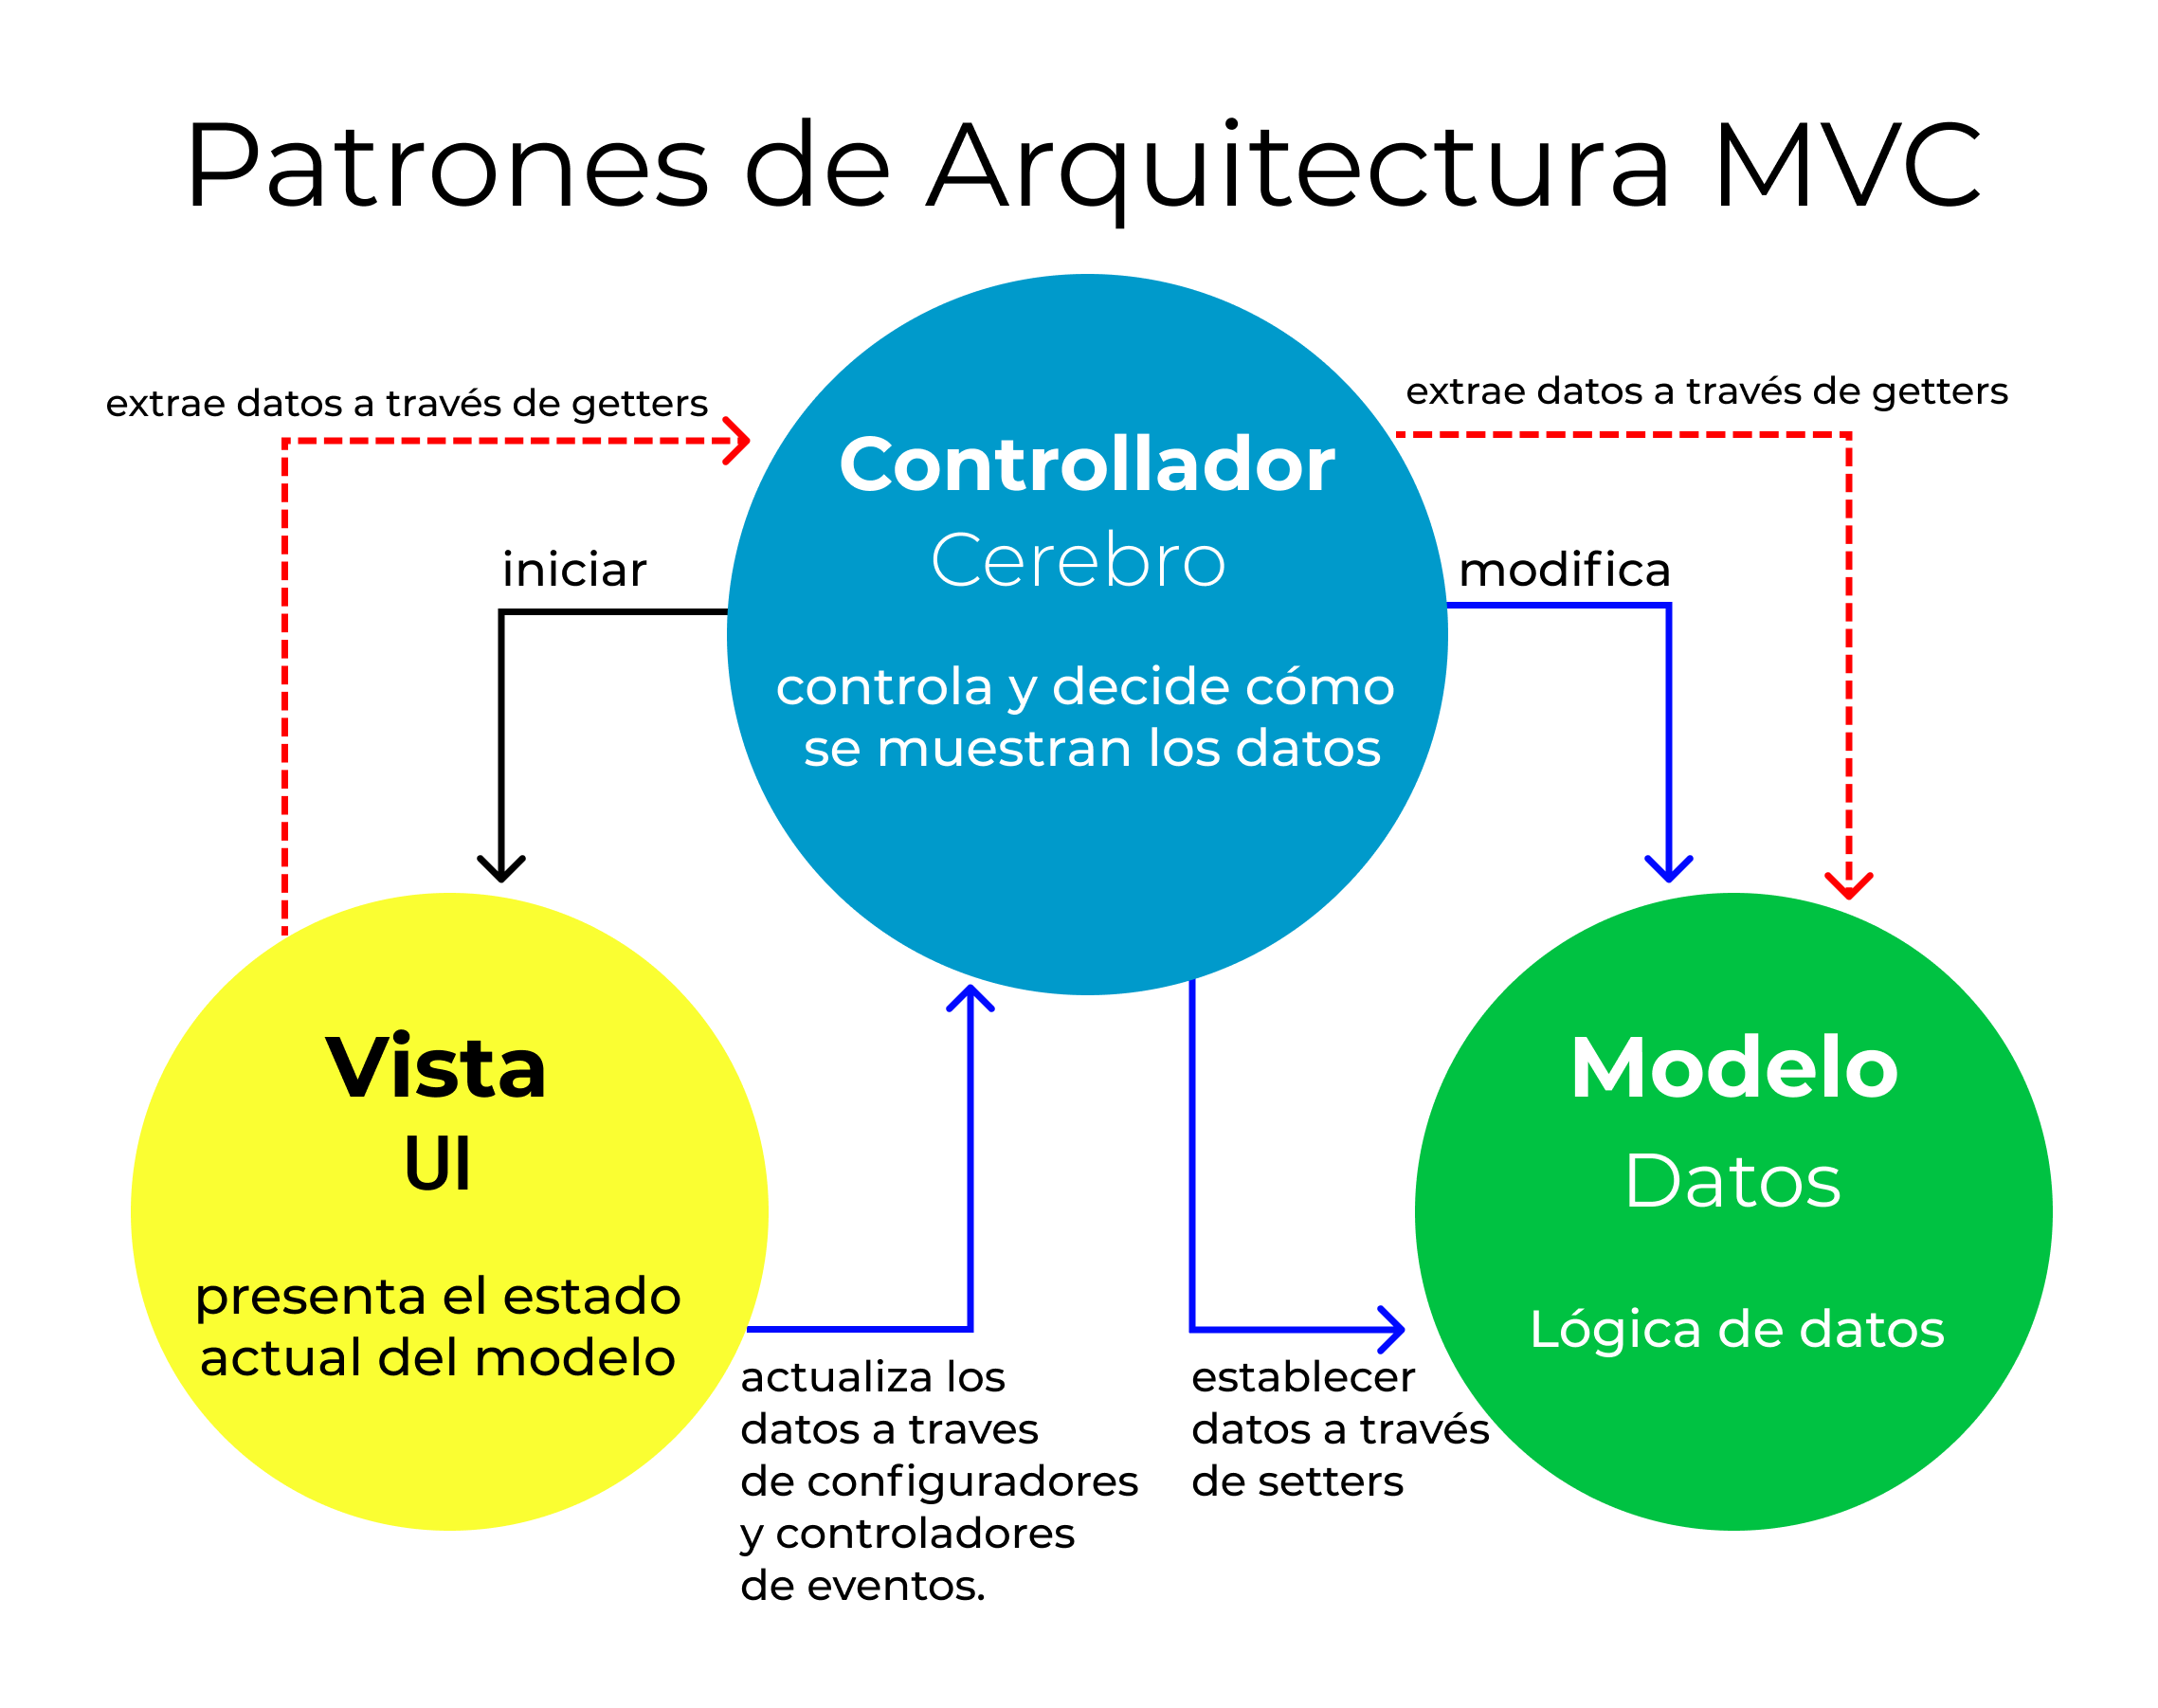
\includegraphics[width=1\linewidth]{img/MVC.png}
    \caption{Patrón Modelo-Vista-Controlador}
    \label{fig:mvc}
\end{figure}

En la aplicación se pueden encontrar estos componentes. En esta aplicación, el modelo para representar los datos obtenidos a través del web scraping o la Web API de Moodle. Este modelo se ve representado en la aplicación en la carpeta situada en src/main/java/es/ubu/lsi/model \ref{fig:modelo}:

\begin{figure}[H]
    \centering
    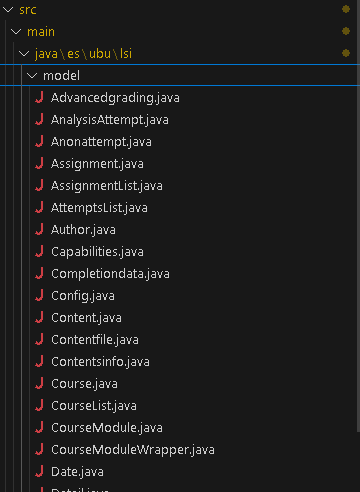
\includegraphics[width=0.6\linewidth]{img/modelo-elearningqa.png}
    \caption{Modelo de eLearningQA}
    \label{fig:modelo}
\end{figure}

La vista se ve representada en ficheros JSP en el paquete src/main/webapp. Aquí, se encuentra la interfaz de usuario y todos los métodos que utiliza. 

El controlador se encuentra en la aplicación\ref{fig:controlador} como un conjunto de clases que realizan las tareas propias a la lógica de negocio.

\begin{figure}[H]
    \centering
    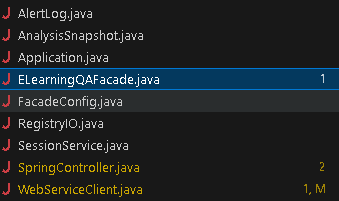
\includegraphics[width=0.5\linewidth]{img/controlador.png}
    \caption{Controlador en eLearningQA}
    \label{fig:controlador}
\end{figure}

Por otro lado, la aplicación cuenta con un patrón fachada, que centraliza los métodos que realizan las operaciones de la aplicación. Este patrón se implementa en la aplicación con una clase fachada llamada ElearningQAFacade que permite el aumento de funcionalidad sin que cambie mucho la fachada de la aplicación \ref{fig:diagrama-clases-elearningqa}.

\begin{figure}[H]
    \centering
    \includegraphics[width=1\linewidth]{patrón-fachada.png}
    \caption{Diagrama de clases de eLearningQA}
    \label{fig:diagrama-clases-elearningqa}
\end{figure}

\section{Diseño de datos}
Esta aplicación no dispone de persistencia de datos en base de datos. Hasta el momento, se guardan datos de los informes en archivos CSV que se utilizan para generar el gráfico de evolución de calidad. 

Sin embargo, sí que existe una gestión de los datos que se reciben desde la Web API de Moodle y del fichero estadístico de la web de Moodle. Estos datos se reciben en formato JSON y se realiza un cast a las entidades definidas en la capa de modelo de la aplicación en la aplicación. 

Las estructura de este Modelo gira en torno al curso, ya que los reportes se generan basándose en el curso. En la siguiente imagen \ref{fig:entidades} se puede ver la estructura de entidades de la que dispone la aplicación.

\begin{figure}[H]
    \centering
    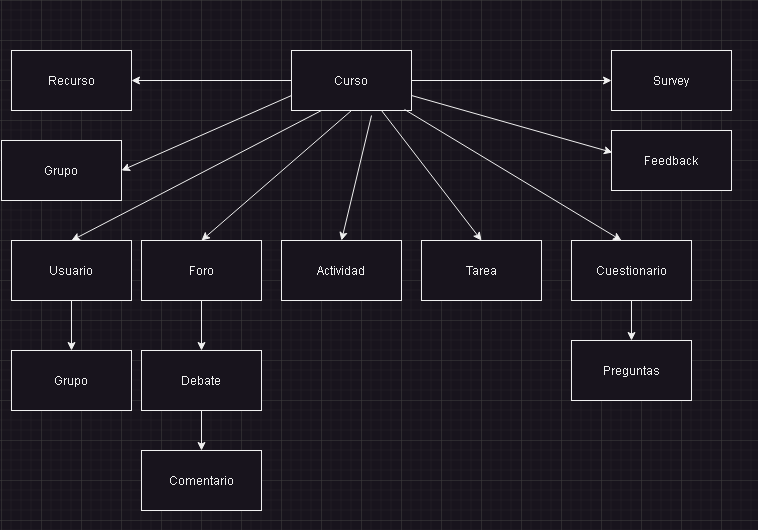
\includegraphics[width=1\linewidth]{img/entidades-modelo.png}
    \caption{Entidades del modelo de eLearningQA}
    \label{fig:entidades}
\end{figure}

\section{Diseño procedimental}
En este apartado se define el diseño procedimental que sigue la aplicación. La funcionalidad principal de la aplicación es la generación de informes de calidad. Para esta funcionalidad existe un conjunto de llamadas a distintos métodos en distintas clases \ref{fig:diseño-procedimental}.

\begin{figure}
    \centering
    \includegraphics[width=1\linewidth]{diseño-procedimental.png}
    \caption{Procedimiento de generación de un informe}
    \label{fig:diseño-procedimental}
\end{figure}

Como conclusión, es importante recalcar que este diseño debe ser revisado constantemente, como parte del proceso del mantenimiento. Ya que basándose en el crecimiento de necesidades, puede ser interesante un cambio estructural con el fin de mejorar le desarrollo de la aplicación en el largo plazo.




\apendice{Documentación técnica de programación}

\section{Introducción}
En este apartado se documentan todos los aspectos importantes para el proceso de programación.

\section{Estructura de directorios}
Este proyecto tiene una estructura de directorios propia de una aplicación Spring Boot MVC \cite{estructura-mvc}, en la que se pueden diferenciar los 3 componentes básicos del patrón Modelo-Vista-Controlador \ref{fig:estructura-elearningqa}.
\begin{figure}[H]
    \centering
    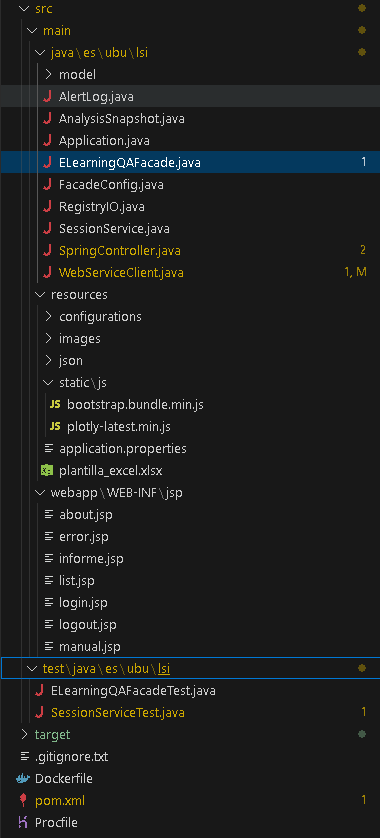
\includegraphics[width=0.6\linewidth]{img/estructura-proyecto.png}
    \caption{Estructura de proyecto de eLearningQA}
    \label{fig:estructura-elearningqa}
\end{figure}

\section{Manual del programador}
Este proyecto está construido con Spring Boot 2.7.18 como framework de desarrollo. Se utiliza Java JDK 8 que se puede descargar de la página oficial \cite{java8}. Para poder desarrollar en este proyecto también se necesita una versión de Apache Maven, la versión utilizada para este desarrollo ha sido la 3.9.6.

El IDE utilizado en este caso ha sido Visual Studio Code, se pueden utilizar otros IDE, el más recomendado para el desarrollo en java es IntelliJ IDEA. 

Para obtener el proyecto se puede acceder al repositorio en GitHub \cite{repositorio}. Hay varias formas de descargar el repositorio, una de ellas es utilizando el comando: 

\begin{verbatim}
git -clone https://github.com/bae1001/eLearningQA
\end{verbatim}

Además, el proyecto cuenta con integración continua con ``Java CI with Maven'', que se utiliza para hacer una comprobación de cada subida al repositorio para verificar que los cambios funcionan correctamente con el conjunto de la aplicación. Para esto existe un fichero de configuración llamado ``maven.yml'' situado en la carpeta de workflows de Github \ref{fig:mvn-ci}.

\begin{figure}[H]
    \centering
    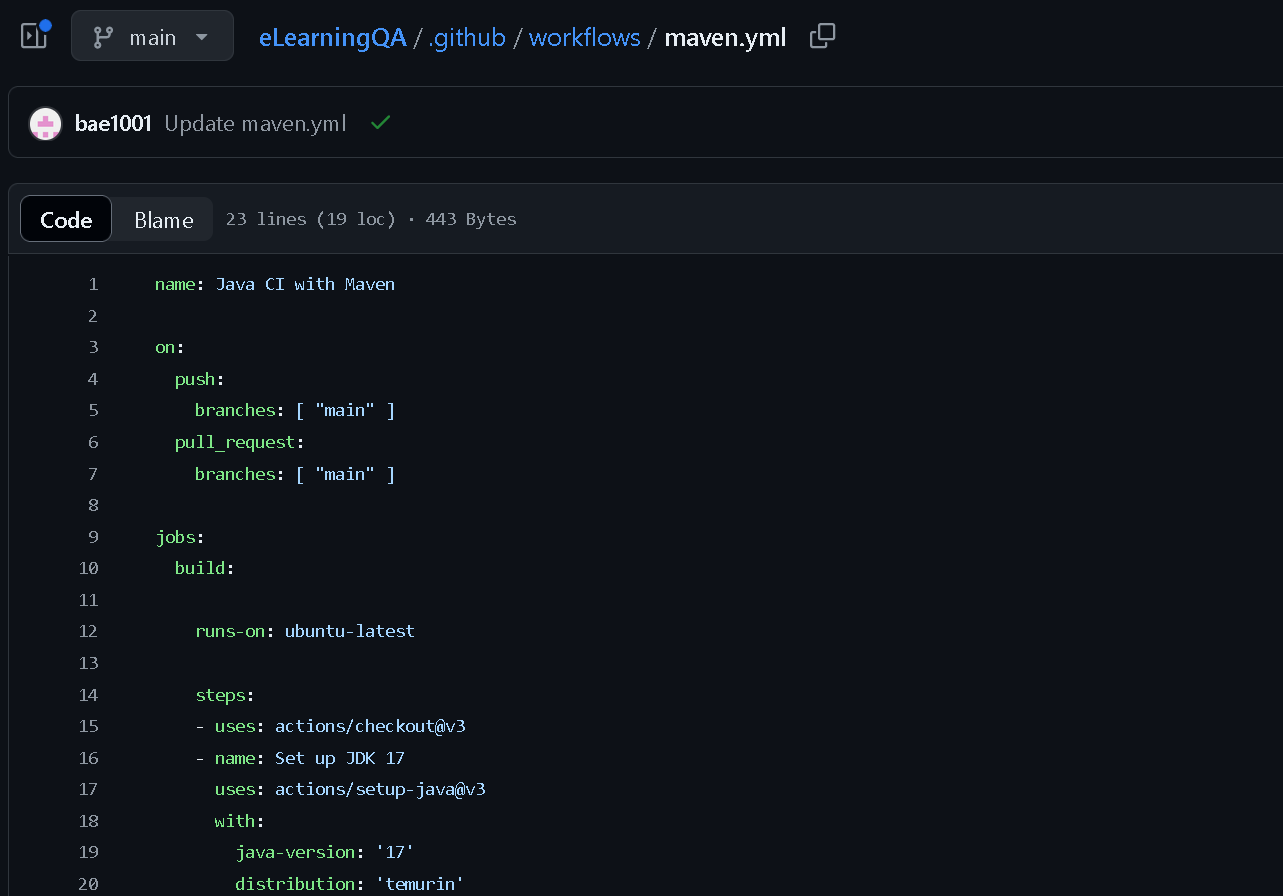
\includegraphics[width=1\linewidth]{img/javaCi_github.png}
    \caption{Fichero de configuración de Java CI with Maven en Github}
    \label{fig:mvn-ci}
\end{figure}

Por otro lado, es necesario disponer de Docker Desktop \cite{docker}, para poder hacer un despliegue en contenedores.

Finalmente, hay que configurar el fichero para la conexión con SonarCloud. Al igual que ``Java CI with Maven'' se debe configurar un fichero en la carpeta de workflows de Github, en este proyecto dicho fichero se llama ``build.yml'' \ref{fig:sonar-workflow}.
\begin{figure}[H]
    \centering
    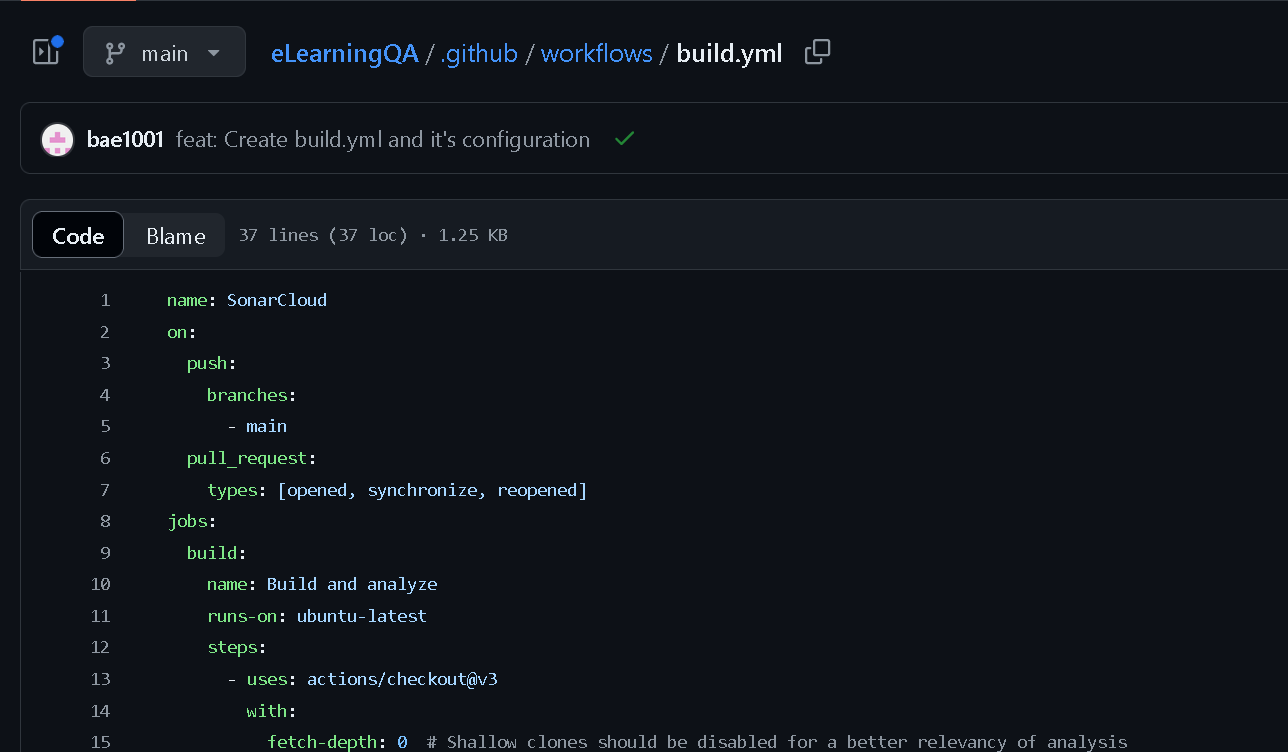
\includegraphics[width=1\linewidth]{img/sonar-workflow.png}
    \caption{Fichero de configuración de Sonarcloud en workflows de Github}
    \label{fig:sonar-workflow}
\end{figure}

\section{Compilación, instalación y ejecución del proyecto}
Para poder ejecutar este proyecto se deben seguir los siguientes pasos:
\begin{enumerate}
    \item Ejecutar el comando de compilación de Maven, a la altura del archivo pom del proyecto:
        \begin{verbatim}
            mvn clean install
        \end{verbatim}
    \item A continuación hay 3 opciones para poner en ejecución el proyecto:
        \begin{enumerate}
            \item Ejecutando el maín situado en la clase Aplication.java situada en el paquete src/main/java/es/ubu/lsi
            \item Ejecutando el .war generado en la compilación:
                \begin{verbatim}
                    java -jar prototipo-0.4-SNAPSHOT.war
                \end{verbatim}
            \item Ejecutando el proyecto en un contenedor de Docker. para ello lo primero será crear la imagen con el siguiente comando:
                \begin{verbatim}
                    docker build -t <nombreDeImagen> .
                \end{verbatim}
            A continuación, se ejecuta la imagen creada con el siguiente comando:
                \begin{verbatim}
                    docker run -p 8080:8080 <nombreDeImagen>
                \end{verbatim}
        \end{enumerate}
        \item A continuación se podrá acceder a la aplicación en localhost en la siguiente dirección:
        \begin{verbatim}
            http://localhost:8080/
        \end{verbatim}
\end{enumerate}


\section{Pruebas del sistema}
Para asegurar la mantenibilidad del proyecto es necesario tener test que aseguren el funcionamiento de las funcionalidades con el paso del tiempo y cuando se modifique código que afecte a dichas funcionalidades. Es una práctica muy recomendable en la calidad de código y conveniente para el desarrollo a largo plazo. Esta aplicación cuenta con test que prueban las funcionalidades principales del proyecto. Estos test se puede encontrar en la carpeta de test del proyecto y se pueden ejecutar manualmente o con el comando de compilación de Maven. 

Estas pruebas utilizan datos de prueba que se encuentran en \textbf{src/main/resources/json}, estos datos se han creado con el fin de cubrir la mayor cantidad de código posible.

\apendice{Documentación de usuario}

\section{Introducción}

\section{Requisitos de usuarios}

\section{Instalación}

\section{Manual del usuario}



\apendice{Anexo de sostenibilización curricular}

\section{Introducción}
Este anexo incluirá una reflexión personal del alumnado sobre los aspectos de la sostenibilidad que se abordan en el trabajo.
Se pueden incluir tantas subsecciones como sean necesarias con la intención de explicar las competencias de sostenibilidad adquiridas durante el alumnado y aplicadas al Trabajo de Fin de Grado.

Más información en el documento de la CRUE \url{https://www.crue.org/wp-content/uploads/2020/02/Directrices_Sosteniblidad_Crue2012.pdf}.

Este anexo tendrá una extensión comprendida entre 600 y 800 palabras.



\bibliographystyle{plain}
\bibliography{bibliografiaAnexos}

\end{document}
